%% LyX 2.4.0~beta5 created this file.  For more info, see https://www.lyx.org/.
%% Do not edit unless you really know what you are doing.
\documentclass[english,footrule]{foils}
\usepackage[T1]{fontenc}
\usepackage[latin9]{inputenc}
\pagestyle{foilheadings}
\setcounter{secnumdepth}{1}
\setcounter{tocdepth}{1}
\usepackage{color}
\usepackage{array}
\usepackage{url}
\usepackage{multirow}
\usepackage{varwidth}
\usepackage{amsmath}
\usepackage{amsthm}
\usepackage{amssymb}
\usepackage{graphicx}

\makeatletter

%%%%%%%%%%%%%%%%%%%%%%%%%%%%%% LyX specific LaTeX commands.
%% Because html converters don't know tabularnewline
\providecommand{\tabularnewline}{\\}
%% Variable width box for table cells
\newenvironment{cellvarwidth}[1][t]
    {\begin{varwidth}[#1]{\linewidth}}
    {\@finalstrut\@arstrutbox\end{varwidth}}

%%%%%%%%%%%%%%%%%%%%%%%%%%%%%% Textclass specific LaTeX commands.
\theoremstyle{definition}
\newtheorem{defn}{\protect\definitionname}
\theoremstyle{plain}
\newtheorem{thm}{\protect\theoremname}

%%%%%%%%%%%%%%%%%%%%%%%%%%%%%% User specified LaTeX commands.
\usepackage{xcolor}
\renewcommand{\labelitemi}{$\textcolor{blue}{\bullet}$}
\renewcommand{\labelitemii}{$\textcolor{teal}{\Rightarrow}$}
\renewcommand{\labelitemiii}{$\textcolor{red}{\rightarrow}$}
\renewcommand{\labelitemiv}{$\textcolor{brown}{\circ}$}
% for French theorems, etc. since I'm using English to fix bullet pb.
\providecommand{\examplename}{Example}
\providecommand{\definitionname}{Definition}
\providecommand{\theoremnname}{Theorem}
\providecommand{\remarkname}{Remark}
\providecommand{\exercisename}{Exercise}
% DT book stuff
\newcommand{\argmin}{\operatornamewithlimits{argmin}} % for a "clean" argmin 
\newcommand{\T}{\mathrm{T}}  % transpose
\newcommand{\PP}{\mathrm{P}}  % probability
\newcommand{\dd}{\mathrm{d}} % integration dx
\newcommand{\ee}{\mathrm{e}} % exponential
\newcommand{\E}{\mathrm{E}} % expectation

\DeclareMathOperator{\Var}{Var}  % for the variance
\DeclareMathOperator{\Cov}{Cov}  % for the covariance
\DeclareMathOperator{\Cor}{Cor}  % for the covariance

%_%_%_%_%_%_%_%_
% for tikz drawings and cartoons
%_%_%_%_%_%_%_%_

\usepackage{tikz}

% for tikzit drawings
\usepackage{tikzit}
\input{flow.tikzstyles}


% for decision trees:
\tikzset{
	treenode/.style = {shape=rectangle, rounded corners,
		draw, align=center,
		top color=white, bottom color=blue!20},
	root/.style     = {treenode, font=\Large, bottom color=red!30},
	env0/.style     = {treenode, font=\large, bottom color=orange!30},
	env1/.style     = {treenode,  bottom color=green!30},
	env/.style      = {treenode, font=\ttfamily\normalsize},
    leaf/.style      = {treenode, font=\ttfamily\normalsize},
	dummy/.style    = {circle,draw}
}
\usetikzlibrary{positioning}

%_%_%_%_%_%_%_%_%_%_
% for algorithms and listings
%_%_%_%_%_%_%_%_%_%_

%\usepackage{algorithm_MA,algpseudocode}
%\usepackage{algorithmic}
\usepackage{algpseudocode}

%\floatstyle{ruled}
%\newfloat{algorithm}{tbp}
%\providecommand{\algorithmname}{Algorithm}
%\floatname{algorithm}{\protect\algorithmname}
%

\usepackage{tcolorbox}


% try and fix \Comment problem due to excessive defs in Chap. DA
\algrenewcommand{\algorithmiccomment}[1]{%
	\hfill$\triangleright$\ \textcolor{darkgray}{#1}}

\makeatother

\usepackage{babel}
\providecommand{\definitionname}{Definition}
\providecommand{\theoremname}{Theorem}

\begin{document}

\MyLogo{SciML - ML methods}
\title{SciML - Machine learning\\
\rule[0.5ex]{1\columnwidth}{3pt}}
\author{Mark Asch - IMU/VLP/CSU }
\date{2023}
\maketitle

\foilhead{Program}

Recall machine learning (ML) techniques for scientific applications
(see \textcolor{blue}{Basic Course} for details):
\begin{enumerate}
\item General principles of ML.
\item \textcolor{red}{Supervised learning:}
\begin{enumerate}
\item Regression.
\item Classification.
\end{enumerate}
\item \textcolor{red}{Unsupervised learning:}
\begin{enumerate}
\item Clustering.
\item Trees.
\end{enumerate}
\item Surrogate models and dimensionality reduction.
\item The use of machine learning in scientific applications.
\item The challenges of applying machine learning to scientific applications.
\end{enumerate}

\foilhead{Classes of ML Methods}
\begin{itemize}
\item \textcolor{magenta}{supervised} learning
\item \textcolor{magenta}{unsupervised} learning
\item reinforcement learning (AlphaGo)
\item self-supervised learning (LLMs, ChatGPT)
\end{itemize}

\foilhead{Review of ML Methods}
\begin{center}
\begin{tabular}{|c|c|c|}
\hline 
Class & Model & Task\tabularnewline
\hline 
\hline 
\multirow{6}{*}{Supervised} & Linear regression & R\tabularnewline
\cline{2-3}
 & CART (trees) & R\&C\tabularnewline
\cline{2-3}
 & SVM & R\&C\tabularnewline
\cline{2-3}
 & NN & R\&C\tabularnewline
\cline{2-3}
 & $k$-NN & C\tabularnewline
\cline{2-3}
 & Naive Bayes & C\tabularnewline
\hline 
\multirow{3}{*}{Unsupervised} & $k$-means & clustering\tabularnewline
\cline{2-3}
 & hierarchical & clustering\tabularnewline
\cline{2-3}
 & PCA & patterns\tabularnewline
\hline 
\end{tabular}
\par\end{center}
\begin{itemize}
\item R = regression, C = classification
\item CART = Classification and Regression Trees
\item SVM = Support Vector Machine
\item NN = Neural Network
\item PCA = Principal Component Analysis
\end{itemize}

\foilhead{$\;$}

\vfill{}

\begin{center}
{\Large\textbf{\textcolor{blue}{SUPERVISED LEARNING}}}{\Large\par}
\par\end{center}

\vfill{}


\foilhead{Linear Regression}
\begin{defn}
[Regression]Regression is an method of \textcolor{magenta}{inferential}
statistics, where we draw evidence and conclusions from measured data
concerning complex, realistic, noisy systems. The goal is to learn
about the relationship between \textcolor{magenta}{covariates} (or
predictors) of interest and \textcolor{magenta}{response} variables
(or outcomes).
\end{defn}
\begin{itemize}
\item Recall: the mathematical framework
\item Suppose that we have:

\begin{itemize}
\item a \textcolor{magenta}{response} variable (to explain), $Y$,
\item $p$ \textcolor{magenta}{explanatory}\footnote{\textcolor{magenta}{Also called: features, attributes}}\textcolor{magenta}{{}
}variables, $X=(X_{1},X_{2},\ldots,X_{p})$,
\item a relationship between $Y$ and $X$ of the form
\[
Y=f(X)+\epsilon
\]
\item where

\begin{itemize}
\item $f$ is an \textcolor{magenta}{unknown} function of $X_{1},X_{2},\ldots,X_{p}$
\item $\epsilon$ is a random \textcolor{magenta}{error} term, independent
of $X,$ and with zero mean
\end{itemize}
\end{itemize}
\item ML is then an ensemble of approaches for \textcolor{magenta}{estimating}
$f$ with the objectives of 

\begin{itemize}
\item \textcolor{magenta}{Prediction}: $\hat{Y}=\hat{f}(X)$ where $\hat{f}$
is an estimation for $f$ and $\hat{Y}$ is the resulting prediction
\item \textcolor{magenta}{Inference}: to understand how $Y$ varies as a
function of $X$ (correlations, importances, linearity, etc.)
\end{itemize}
\item Linear regression is a special case, where we suppose that the response,
$Y,$ depends \textcolor{magenta}{linearly} on the unknown \textcolor{magenta}{coefficients}.
In other words, we suppose that
\[
\mathbf{Y}=\mathbf{X}\boldsymbol{\beta}+\boldsymbol{\epsilon}
\]
\item Linear regression is the\textcolor{magenta}{{} workhorse} of statistics!
\item Note that LR is linear in the coeffcients, \textcolor{magenta}{not}
in the predictors that can have completely general, \textcolor{red}{nonlinear}
forms.
\end{itemize}

\foilhead{Linear Regression - Assumptions}
\begin{itemize}
\item Recall: typical \textcolor{magenta}{assumptions} for a (S)LR model
are
\begin{itemize}
\item \textbf{A1}: The model is linear: e.g. $y_{i}=f(x;\beta)+\epsilon_{i}=\beta_{0}+\beta_{1}x_{1}+\epsilon_{i}$ 
\item \textbf{A2}: Unbiased errors: $\mathbb{E}[\epsilon_{i}|x_{i}]=\mathbb{E}[\epsilon_{i}]=0$ 
\item \textbf{A3}: Uncorrelated errors: $\Cov(\epsilon_{i},\epsilon_{j})=0$
for $i\neq j$. 
\item \textbf{A4}: Constant variance: $\Var[y_{i}|x_{i}]=\sigma^{2}$ 
\item \textbf{A5}: Probability distribution: e.g. $\epsilon_{i}\stackrel{\mathrm{iid}}{\sim}\mathcal{N}(0,\sigma^{2})$. 
\item \textbf{A6}: Representative sampling that generalizes to the population---see
\textcolor{blue}{Bias and Ethics Lectures}.
\end{itemize}
\end{itemize}

\foilhead{Linear Regression - Popularity}
\begin{itemize}
\item \textcolor{magenta}{Easy} to implement (just matrix linear algebra)
and \textcolor{magenta}{fast} to compute.
\item Solid \textcolor{magenta}{theoretical} foundation providing full array
of \textcolor{magenta}{diagnostic} tools.
\item Straightforward \textcolor{magenta}{interpretations}----we obtain
an \textcolor{red}{explicit formula}!
\item Surprisingly \textcolor{magenta}{flexible} and adaptable, though may
require some empirical modelling, prior knowledge, experience.
\item Provides good \textcolor{magenta}{approximations} in many cases.
\end{itemize}

\foilhead{Multiple Linear Regression}
\begin{itemize}
\item Linear regression is a fundamental statistical method used for modeling
the relationship between a dependent variable (often denoted as \textquotedbl$y$\textquotedbl )
and one or more independent variables (often denoted as \textquotedbl$X$\textquotedbl ). 
\item It assumes that this relationship can be approximated by a \textcolor{magenta}{linear
equation} of the form
\[
\mathbf{y}=\beta_{0}+\beta_{1}\mathbf{X}_{1}+\beta_{2}\mathbf{X}_{2}+\ldots+\beta_{p}\mathbf{X}_{p}+\boldsymbol{\epsilon}
\]
where 
\begin{itemize}
\item $\mathbf{y}\in\mathbb{R}^{n}$ is the dependent variable (the one
you want to predict), containing $n$ observations, $y_{1},\ldots,y_{n}$
\item $\mathbf{X}_{1},\mathbf{X}_{2},\ldots,\mathbf{X}_{p}$ are the independent
variables or features, with each $\mathbf{X}_{j}\in\mathbb{R}^{n}$
for $j=1,\ldots,p.$
\item $\beta_{0},\beta_{1},\ldots,\beta_{p}$ are the coefficients of the
linear equation that need to be estimated. 
\item $\boldsymbol{\epsilon}\in\mathbb{R}^{n}$ represents the error term,
which accounts for the variability in $\mathbf{y}$ that cannot be
explained by the linear relationship with the $\mathbf{X}$ variables.
\end{itemize}
\item In matrix-vector form, this equation can be written as
\[
\mathbf{y}=\mathbf{X}\boldsymbol{\mathbf{\beta}}+\boldsymbol{\epsilon}
\]
where: 
\begin{itemize}
\item $\mathbf{y}$ is a column vector with dimension $n\times1$ of the
\textcolor{magenta}{dependent} variable values. 
\item $\mathbf{X}$ is the \textcolor{magenta}{design matrix} , of dimension
$n\times(p+1)$ where each row represents one observation and each
column represents an independent variable. 
\item $\boldsymbol{\mathbf{\beta}}$ is a column vector, dimension $(p+1)\times1,$
of the \textcolor{magenta}{coefficient} estimates, including $\beta_{0}$
\item $\boldsymbol{\epsilon}$ is IID, centered Gaussian\footnote{The Gaussian noise model is NOT restrictive, but is the most arbitrary
one with the least number of hypotheses. We only assume centrality
and decreasing probability of large and small values. } noise with $\E(\boldsymbol{\epsilon})=0$ and $\Cov(\boldsymbol{\epsilon})=\sigma^{2}\mathbf{I}$,
sometimes written as $\epsilon_{i}\stackrel{\mathrm{iid}}{\sim}(0,\sigma^{2})$
\end{itemize}
\item Writing this out, we obtain
\begin{align*}
\mathbf{y} & =\left[\begin{array}{c}
y_{1}\\
\vdots\\
y_{n}
\end{array}\right],\quad\mathbf{X}=\left[\begin{array}{cccc}
1 & x_{11} & \hdots & x_{1p}\\
\vdots & \vdots & x_{ij} & \vdots\\
1 & x_{n1} & \hdots & x_{np}
\end{array}\right],\\
 & \quad\boldsymbol{\beta}=\left[\begin{array}{c}
\beta_{0}\\
\vdots\\
\beta_{p}
\end{array}\right],\quad\mathbf{\epsilon}=\left[\begin{array}{c}
\epsilon_{1}\\
\vdots\\
\epsilon_{n}
\end{array}\right]
\end{align*}
 or in the SLR case,
\end{itemize}
\[
\underbrace{\vphantom{\begin{bmatrix}1 & x_{1}\\
1 & x_{2}\\
\vdots~ & \vdots\\
1 & x_{n}
\end{bmatrix}}\begin{bmatrix}~y_{1}\\
~y_{2}\\
\vdots\\
y_{n}
\end{bmatrix}}_{{\textstyle \begin{gathered}\mathbf{y}\end{gathered}
}}=\underbrace{\begin{bmatrix}1 & x_{1}\\
1 & x_{2}\\
\vdots~ & \vdots\\
1 & x_{n}
\end{bmatrix}}_{{\textstyle \begin{gathered}=\mathbf{X}\end{gathered}
}}\underbrace{\vphantom{\begin{bmatrix}1 & x_{1}\\
1 & x_{2}\\
\vdots~ & \vdots\\
1 & x_{n}
\end{bmatrix}}\begin{bmatrix}\beta_{0}\\
\beta_{1}
\end{bmatrix}}_{{\textstyle \begin{gathered}\boldsymbol{\beta}\end{gathered}
}}+\underbrace{\vphantom{\begin{bmatrix}1 & x_{1}\\
1 & x_{2}\\
\vdots~ & \vdots\\
1 & x_{n}
\end{bmatrix}}\begin{bmatrix}\epsilon_{1}\\
\epsilon_{2}\\
\vdots\\
\epsilon_{n}
\end{bmatrix}}_{{\textstyle \begin{gathered}+\boldsymbol{\epsilon}\end{gathered}
}}
\]

\begin{itemize}
\item In multiple linear regression, the coefficients (also known as the
parameter estimates) are computed, as in simple linear regression,
using a method called \textcolor{magenta}{ordinary least squares}
(OLS). 
\begin{itemize}
\item The goal of OLS is to \textcolor{magenta}{minimize} the sum of squared
errors (SSE), which is the sum of the squared differences between
the observed $\mathbf{y}$ values and the predicted $\mathbf{y}$
values. 
\item Mathematically, this is represented as,
\[
\mathrm{SSE}=\sum_{i=1}^{n}(y_{i}-\hat{y}_{i})^{2}
\]
where $\hat{y}_{i}$ is the predicted value of $y$ for the $i$-th
observation.
\end{itemize}
\item The \textcolor{magenta}{optimal solution }of this minimization problem
can in fact be derived explicitly, and is quite easily shown to be
given by
\[
\boldsymbol{\beta}_{\mathrm{LS}}=\left(\mathbf{X}^{\mathrm{T}}\mathbf{X}\right)^{-1}\mathbf{X}^{\mathrm{T}}\mathbf{y}
\]
\end{itemize}

\foilhead{Recall: Noise Model}
\begin{itemize}
\item A noise model is essential for any analysis, particularly \textcolor{magenta}{Bayesian}
(of which regression is an example)
\item \textcolor{magenta}{Neutrality} of the Gaussian hypothesis for the
noise model:
\begin{itemize}
\item the noise is centered : its mean value is zero, but it can take any
value (small or big)
\item large amplitudes/deviations are less and less probables: the variance
is finite
\item independence between observations (otherwise, this is part of the
trends of the model)
\end{itemize}
\item We neither suppose, nor impose that the noise really follows a \textcolor{magenta}{Gaussian}
law...
\end{itemize}

\foilhead{Linear Regression: Diagnostics}
\begin{itemize}
\item The only ML method with complete diagnostics:
\begin{itemize}
\item \textcolor{magenta}{Coefficient of determination} \textcolor{magenta}{(R-squared)}
\[
R^{2}=1-\frac{\sum_{i}\left(y_{i}-\hat{y}_{i}\right)^{2}}{\sum_{i}\left(y_{i}-\bar{y}\right)^{2}}=1-\frac{\mathrm{RSS}}{\mathrm{TSS}}=\frac{\mathrm{TSS}-\mathrm{RSS}}{\mathrm{TSS}}
\]
represents the proportion of the variance ``explained'' by the model.
Beware of the \textcolor{magenta}{limitations} of this coefficient!
\item \textcolor{magenta}{Mean-squared Error}:
\[
\mathrm{MSE}=\frac{1}{n}\sum_{i=1}^{n}\left(y_{i}-\hat{y}_{i}\right)^{2}.
\]
Can be more reliable than R-squared, but is context-dependent (not
between $0$ and $1$).
\item \textcolor{magenta}{p-values} and significance: these are no longer
considered to be advisable, and in general should not be used.
\end{itemize}
\item \textcolor{magenta}{Graphical} diagnostics
\begin{enumerate}
\item The plots (``\textcolor{magenta}{Residuals vs Fitted}'' and ``Scale-Location'')
should not give any clear trends (they should neither be all increasing
or all decreasing). This shows:
\begin{enumerate}
\item that on average, the regression line is well fitted to the data, and
thus the hypothesis of linearity is acceptable,
\item that the variance is constant and of the same value for all the observations.
\end{enumerate}
\item The \textcolor{magenta}{``normal Q-Q}'' plot should show points
distributed around the dashed line and that follow the line approximately,
without marked deviations (especially at the extremities). This shows
that the hypothesis of the residues having a normal distribution,
is satisfied.
\item The last ``\textcolor{magenta}{Cook distances}'', should not show
any point that exceeds 1 on the abscissa. This shows the presence
of influential data.
\end{enumerate}
\end{itemize}
\begin{center}
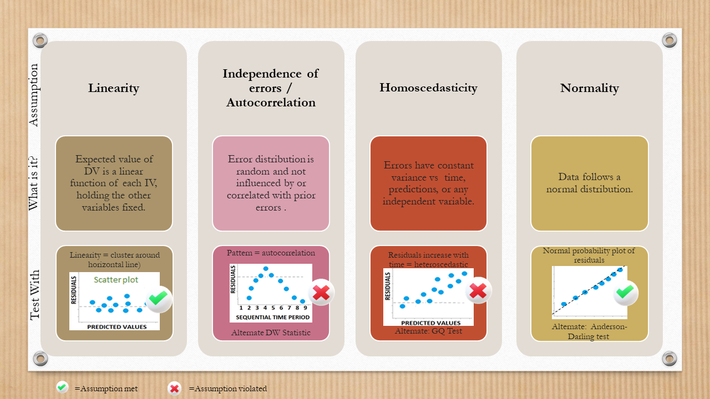
\includegraphics[width=1\textwidth]{graphics/lin_reg_assump}
\par\end{center}

\begin{center}
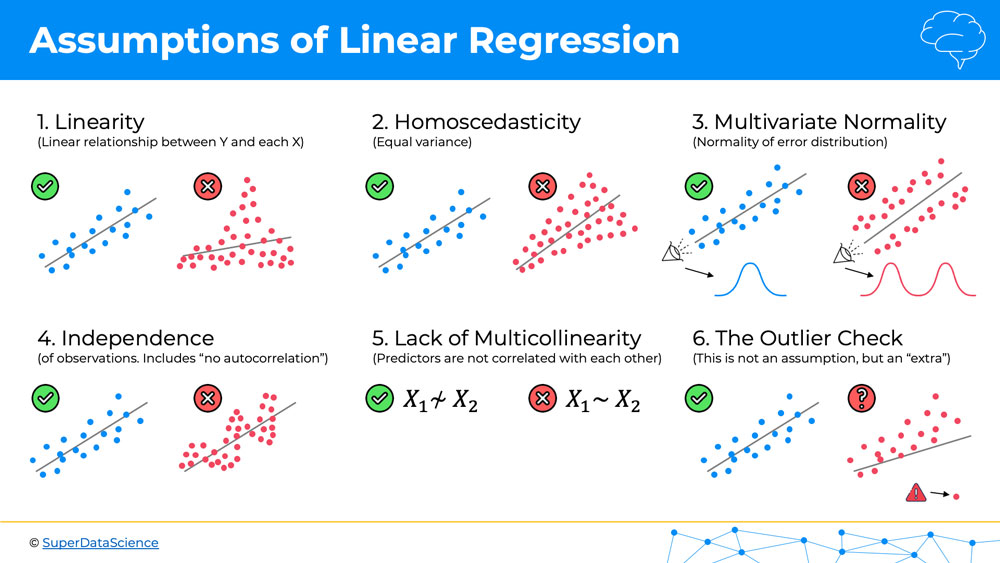
\includegraphics[width=1\textwidth]{graphics/LRassumps}
\par\end{center}

\begin{center}
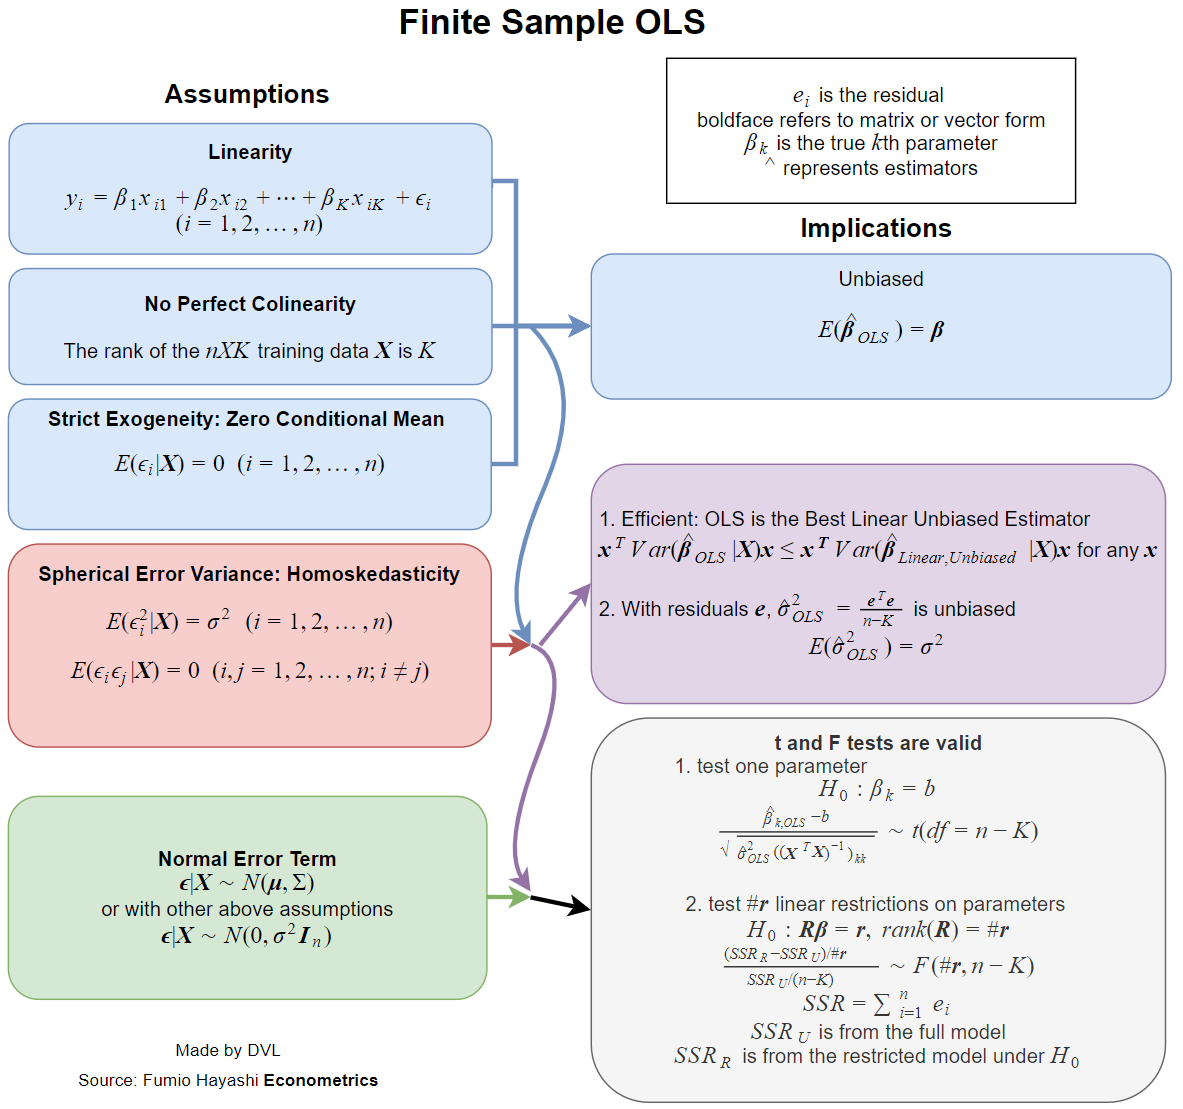
\includegraphics[width=1\textwidth]{graphics/finite_sample_OLS}
\par\end{center}

\foilhead{Recall: Simple Linear Regression Model}
\begin{itemize}
\item \textbf{\textcolor{magenta}{L}}inear Function: The mean of the response,
$\mbox{E}(Y_{i}),$ at each value of the predictor, $x_{i},$ is a
Linear function of the $x_{i}.$ 
\item \textbf{\textcolor{magenta}{I}}ndependent: The errors, $\epsilon_{i},$
are Independent.
\item \textbf{\textcolor{magenta}{N}}ormally Distributed: The errors, $\epsilon_{i},$
at each value of the predictor, $x_{i},$ are Normally distributed.
\item \textbf{\textcolor{magenta}{E}}qual variances (denoted $\sigma^{2}$
): The errors, $\epsilon_{i},$ at each value of the predictor, $x_{i},$
have Equal variances (denoted $\sigma^{2}$ ).
\end{itemize}

\foilhead{Regression: Shrinkage and Selection}
\begin{itemize}
\item \textbf{Prediction}:
\begin{itemize}
\item Linear regression: $E(Y_{j}|X)=X\beta$;
\item Or for a more general regression function: $E(Y_{j}|X)=f(X)$;
\item In a prediction context, there is less concern about the values of
the components of the right-hand side, rather interest is on the total
contribution.
\end{itemize}
\item \textbf{Variable Selection}:
\begin{itemize}
\item The driving force behind variable selection:
\begin{itemize}
\item The desire for a parsimonious regression model (one that is simpler
and easier to interpret);T
\item he need for greater accuracy in prediction.
\end{itemize}
\item The notion of what makes a variable \textquotedbl important\textquotedbl{}
is still not well understood, but one interpretation (Breiman, 2001)
is that a variable is important if dropping it seriously affects prediction
accuracy.
\item Selecting variables in regression models is a complicated problem,
and there are many conflicting views on which type of variable selection
procedure is best, e.g. LRT, F-test, AIC, and BIC.
\end{itemize}
\item There are two main types of \textbf{stepwise procedures} in regression:
\begin{itemize}
\item Backward elimination: eliminate the least important variable from
the selected ones.
\item Forward selection: add the most important variable from the remaining
ones.
\item A hybrid version that incorporates ideas from both main types: alternates
backward and forward steps, and stops when all variables have either
been retained for inclusion or removed.
\end{itemize}
\item \textbf{Criticisms} of Stepwise Methods:
\begin{itemize}
\item There is no guarantee that the subsets obtained from stepwise procedures
will contain the same variables or even be the \textquotedbl best\textquotedbl{}
subset.
\item When there are more variables than observations ($p>n$), backward
elimination is typically not a feasible procedure.
\item The maximum or minimum of a set of correlated F statistics is not
itself an F statistic.
\item It produces a single answer (a very specific subset) to the variable
selection problem, although several different subsets may be equally
good for regression purposes.
\item The computing is easy by the use of R function \texttt{\textcolor{blue}{step()}}
or \texttt{\textcolor{blue}{regsubsets()}}. However, to specify a
practically good answer, you must know the practical context in which
your inference will be used.
\end{itemize}
\end{itemize}

\foilhead{Linear Regression: LASSO and Ridge}
\begin{itemize}
\item Ridge regression and Lasso regression are two popular regularization
techniques used in linear regression to address issues such as multicollinearity,
feature selection and overfitting. 
\end{itemize}
\textbf{Motivation:} ill-conditioned $X$
\begin{itemize}
\item Because the LS estimates depend upon $(X^{\mathrm{T}}X)^{-1},$ we
would have problems in computing $\beta_{LS}$ if $X^{\mathrm{T}}X$
were singular or nearly singular.
\item In those cases, small changes to the elements of $X$ lead to large
changes in $(X^{\mathrm{T}}X)^{-1},$
\item The least square estimator $\beta_{\mathrm{LS}}$ i may provide a
good fit to the training data, but it will not fit sufficiently well
to the test data.
\end{itemize}

\foilhead{Linear Regression: Ridge}

\textbf{Objective}: 
\begin{itemize}
\item \textcolor{magenta}{Ridge regression}, also known as L2 regularization,
aims to prevent multicollinearity by adding a penalty term to the
linear regression objective function. 
\item The objective is to find the values of coefficients $\boldsymbol{\beta}$
that minimize the following modified sum of squared errors,
\[
\mathrm{SSE_{\text{Ridge}}}=\sum_{i=1}^{n}(y_{i}-\hat{y}_{i})^{2}+\lambda\sum_{j=1}^{p}\beta_{j}^{2}
\]
where 
\begin{itemize}
\item the second term, $\lambda\sum_{j=1}^{p}\beta_{j}^{2}$, is the \textcolor{magenta}{regularization}
term. 
\item $\lambda$ (lambda) is the regularization parameter, which controls
the \textcolor{magenta}{strength} of regularization
\item this is a \textcolor{magenta}{hyperparameter} and needs to be tuned:
\begin{itemize}
\item If we choose $\lambda=0,$ we have $p$ parameters (since there is
no penalization).
\item If $\lambda$ is large, the parameters are strongly constrained and
the degrees of freedom will effectively be lower, tending to $0$
as $\lambda\rightarrow\infty.$ 
\item We need to choose a value inbetween...
\end{itemize}
\end{itemize}
\end{itemize}
\textbf{Effect}: 
\begin{enumerate}
\item Ridge regression \textcolor{magenta}{shrinks the coefficients} towards
zero but doesn't eliminate them entirely. 
\item It is effective in preventing \textcolor{magenta}{multicollinearity}
by encouraging smaller coefficient values.
\end{enumerate}

\foilhead{Linear Regression: LASSO }

\textbf{Objective}: 
\begin{itemize}
\item \textcolor{magenta}{Lasso regression}, also known as L1 regularization,
not only prevents multicollinearity but also performs \textcolor{magenta}{feature
selection} by adding a penalty term to the linear regression objective
function. 
\item The objective is to find the values of coefficients $\beta$ that
minimize the following modified sum of squared errors,
\[
\mathrm{SSE_{\text{Lasso}}}=\sum_{i=1}^{n}(y_{i}-\hat{y}_{i})^{2}+\lambda\sum_{j=1}^{p}|\beta_{j}|
\]
where
\begin{itemize}
\item $\mathrm{SSE_{\text{Lasso}}}$ is the sum of squared errors with a
\textcolor{magenta}{regularization} term. 
\item The second term, $\lambda\sum_{j=1}^{p}|\beta_{j}|$, is the \textcolor{magenta}{regularization}
term with the absolute values of coefficients.
\end{itemize}
\end{itemize}
\textbf{Effect}: 
\begin{enumerate}
\item Lasso regression encourages \textcolor{magenta}{sparsity}, meaning
it tends to force some coefficients to be exactly zero, effectively
removing irrelevant features from the model. 
\item It is useful when you have a large number of features and want automatic
\textcolor{magenta}{feature selection}. As $p$ increases, the multidimensional
diamond, described by the L1 norm, has an increasing number of corners,
and so it is highly likely that some coefficients will be set equal
to zero. Hence, the lasso performs \textcolor{magenta}{shrinkage}
and (effectively) subset \textcolor{magenta}{selection}.
\end{enumerate}

\foilhead{Regression - Generalizations}
\begin{itemize}
\item generalized linear models GLM
\item categorical predictors
\item spline regressions (MARS)
\end{itemize}

\foilhead{Classification---simple/linear}

\begin{tcolorbox}[colback=red!5!white,colframe=red!75!black,title=Note] 
Please review this material in the Basic Course.
\end{tcolorbox}
\begin{itemize}
\item k-NN:
\begin{itemize}
\item The only parameter that can adjust the complexity of k-NN is the number
of neighbors $k.$
\item The larger $k$ is, the smoother the classification boundary. 
\item Or we can think of the complexity of k-NN as lower when $k$ increases.
\end{itemize}
\item Logistic, Naive Bayes, LDA
\item nonlinear methods---see below
\end{itemize}

\foilhead{Applyng k-NN in Practice}

If you wish to apply k-NN in practice proceed as follows:
\begin{enumerate}
\item \textcolor{magenta}{Preprocess} your data: Normalize the features
in your data (e.g. one pixel in images) to have zero mean and unit
variance. We will cover this in more detail in later sections, and
chose not to cover data normalization in this section because pixels
in images are usually homogeneous and do not exhibit widely different
distributions, alleviating the need for data normalization.
\item If your data is very high-dimensional, consider using a \textcolor{magenta}{dimensionality
reduction} technique such as PCA, NCA, or even Random Projections.
\item \textcolor{magenta}{Split} your training data randomly into train/val
splits. 
\begin{enumerate}
\item As a rule of thumb, between 70-90\% of your data usually goes to the
train split. 
\item This setting depends on how many hyperparameters you have and how
much of an influence you expect them to have. 
\item If there are many hyperparameters to estimate, you should err on the
side of having larger validation set to estimate them effectively.
\item If you are concerned about the size of your validation data, it is
best to split the training data into folds and perform cross-validation. 
\item If you can afford the computational budget it is always safer to go
with cross-validation (the more folds the better, but more expensive).
\end{enumerate}
\item \textcolor{magenta}{Train and evaluate} the k-NN classifier on the
validation data (for all folds, if doing cross-validation) 
\begin{enumerate}
\item for many choices of k (e.g. the more the better) and 
\item across different distance types (L1 and L2 are good candidates)
\end{enumerate}
\item If your k-NN classifier is running too long, consider using an Approximate
Nearest Neighbor library (e.g. FLANN) to accelerate the retrieval
(at cost of some accuracy).
\item Take note of the \textcolor{magenta}{hyperparameters} that gave the
best results. 
\begin{enumerate}
\item There is a question of whether you should use the full training set
with the best hyperparameters, since the optimal hyperparameters might
change if you were to fold the validation data into your training
set (since the size of the data would be larger). 
\item In practice it is cleaner to not use the validation data in the final
classifier and consider it to be burned on estimating the hyperparameters.
Evaluate the best model on the test set. 
\item Report the \textcolor{red}{test set accuracy} and declare the result
to be the performance of the k-NN classifier on your data.
\end{enumerate}
\end{enumerate}

\foilhead{Support Vector Machines}
\begin{itemize}
\item The support vector machine (SVM) algorithm performs \textcolor{magenta}{supervised
classification}. 
\item It can provide \textcolor{magenta}{excellent performance} in a broad
range of contexts.
\item It is considered to be one of the foremost ``\textcolor{magenta}{black
box}'' methods of statistical learning---see \textcolor{blue}{Bias
and Ethics Lectures}. 
\item The basic property of the algorithm is its generalization of the boundary
between classes to \textcolor{magenta}{nonlinear} curves and hypersurfaces.
\item Please refer to the \textcolor{blue}{Basic Course} for full explanation
and details.
\end{itemize}

\foilhead{SVM in a nutshell}
\begin{itemize}
\item The SVM algorithm looks for a \textcolor{magenta}{linearly separable
hyperplane}, or a \textcolor{magenta}{decision boundary} separating
members of one class from the other. 
\begin{itemize}
\item If such a hyperplane exists, the work is done! 
\item If such a hyperplane does not exist, SVM uses a \textcolor{magenta}{nonlinear
mapping} to transform the training data into a higher dimension. 
\end{itemize}
\item Then it searches for the linear optimal separating hyperplane. 
\begin{itemize}
\item With an appropriate nonlinear mapping to a sufficiently high dimension,
data from two classes can \textcolor{magenta}{always }be separated
by a hyperplane. 
\item The SVM algorithm finds this hyperplane using \textcolor{magenta}{support
vectors }and \textcolor{magenta}{margins}. 
\end{itemize}
\item As a training algorithm, SVM may not be very fast compared to some
other classification methods, but owing to its ability to model complex
nonlinear boundaries, SVM has \textcolor{magenta}{high accuracy}. 
\item SVM is comparatively less prone to \textcolor{magenta}{overfitting}. 
\item SVM has \textcolor{magenta}{successfully} been applied to handwritten
digit recognition, text classification, speaker identification etc.
\end{itemize}

\foilhead{SVM for Regression}
\begin{itemize}
\item We can use SVM to perform \textcolor{magenta}{regressions} too. 
\item Instead of computing the coefficients $\beta_{i}$ to minimize the
SLR least squares criterion on the residuals, SVM imposes a\textcolor{magenta}{{}
modified loss}. 
\item This loss uses only residuals that are larger in absolute value than
a given positive constant. 
\item The loss function is defined as 
\[
L(y,\hat{y})=\begin{cases}
0 & \mathrm{if}\,\left|y-\hat{y}\right|<\epsilon,\\
\left|y-\hat{y}\right|-\epsilon & \mathrm{otherwise},
\end{cases}
\]
implying that any point lying within an \textcolor{magenta}{$\epsilon$-neighborhood}---or
tube---around the prediction is not penalized. 
\item This is related to \textcolor{magenta}{LASSO} regression presented
above. 
\item This gives an advantage over classical least squares regression, in
that we can fit extremely nonlinear functions, such as those that
exhibit \textcolor{magenta}{saturation} and \textcolor{magenta}{thresholding}.
\end{itemize}

\foilhead{Decision Trees and Random Forests}
\begin{itemize}
\item \textbf{Background}:
\begin{itemize}
\item Decision tree learning is a method for approximating \textcolor{magenta}{discrete-valued}
target functions, in which the learned function is represented by
a decision tree. 
\item Learned trees can also be re-represented as sets of\textcolor{magenta}{{}
if-then rules }to improve human readability. 
\item These learning methods are among the most popular of \textcolor{magenta}{inductive
inference} algorithms 
\item They have been successfully applied to a \textcolor{magenta}{broad
range }of tasks from learning to diagnose medical cases to learning
to assess credit risk of loan applicants.
\item Classification trees are a \textcolor{magenta}{hierarchical} way of
partitioning the space. We start with the entire space and recursively
divide it into smaller regions. In the end, every region is assigned
to a class label.
\end{itemize}
\item \textbf{Recall}:
\begin{itemize}
\item Decision trees can be applied to both \textcolor{magenta}{classification}
and \textcolor{magenta}{regression} problems.
\item They are particularly clear to interpret, but suffer from a lack of
\textcolor{magenta}{robustness}.
\item Random Forests (RF), bagging and boosting repair the robustness and
are extremely good classifiers and regressors.
\end{itemize}
\item To go further, we need to study:
\begin{itemize}
\item pruning - usually done by cross-validation
\item bagging
\item boosting
\item RF and \textcolor{magenta}{variable importance} for model reduction/feature
selection.
\end{itemize}
\end{itemize}

\foilhead{Random Forests}
\begin{itemize}
\item Bagging---bootstrap aggregation---constructs a large number of trees
with \textcolor{magenta}{bootstrap} samples from a dataset. 
\item For RF, as each tree is constructed, take a \textcolor{magenta}{random
sample} of predictors before each node is split. 
\begin{itemize}
\item For example, if there are twenty predictors, choose a random five
as candidates for constructing the best split. 
\item Repeat this process for each node until the tree is large enough.
And as in bagging, do not prune.
\end{itemize}
\item Why do RFs work?
\begin{itemize}
\item \textcolor{magenta}{Variance} reduction: 
\begin{itemize}
\item The trees are more independent because of the combination of bootstrap
samples and random draws of predictors.
\item It is apparent that random forests are a form of bagging, and the
averaging over trees can substantially reduce instability that might
otherwise result. Moreover, by working with a random sample of predictors
at each possible split, the fitted values across trees are more independent.
Consequently, the gains from averaging over a large number of trees
(variance reduction) can be more dramatic.
\end{itemize}
\item \textcolor{magenta}{Bias} reduction: 
\begin{itemize}
\item A very large number of predictors can be considered, and local feature
predictors can play a role in tree construction.
\item Random forests are able to work with a very large number of predictors,
even with more predictors than there are observations. An obvious
gain with random forests is that more information may be brought to
reduce bias of fitted values and estimated splits.
\item There are often a few predictors that \textcolor{magenta}{dominate}
the decision tree fitting process because on the average they consistently
perform just a bit better than their competitors. Consequently, many
other predictors, which could be useful for very local features of
the data, are rarely selected as splitting variables. With random
forests computed for a large enough number of trees, each predictor
will have at least several opportunities to be the predictor defining
a split. In those opportunities, it will have very few competitors.
Much of the time a dominant predictor will not be included. Therefore,
local feature predictors will have the opportunity to define a split.
\end{itemize}
\end{itemize}
\item Indeed, random forests are among the very \textcolor{magenta}{best
classifiers }invented to date (Breiman, 2001).
\item Random forests include 3 main \textcolor{magenta}{tuning} parameters.
\begin{enumerate}
\item Node Size: unlike in decision trees, the number of observations in
the terminal nodes of each tree of the forest can be very small. The
goal is to grow trees with as little bias as possible.
\item Number of Trees: in practice, 500 trees is often a good choice.
\item Number of Predictors Sampled: the number of predictors sampled at
each split would seem to be a key tuning parameter that should affect
how well random forests perform. Sampling 2-5 each time is often adequate.
\end{enumerate}
\end{itemize}

\foilhead{$\;$}

\vfill{}

\begin{center}
{\Large\textbf{\textcolor{blue}{SUPERVISED LEARNING - Neural Networks}}}{\Large\par}
\par\end{center}

\vfill{}


\foilhead[-0.5in]{Neural Networks}
\begin{center}
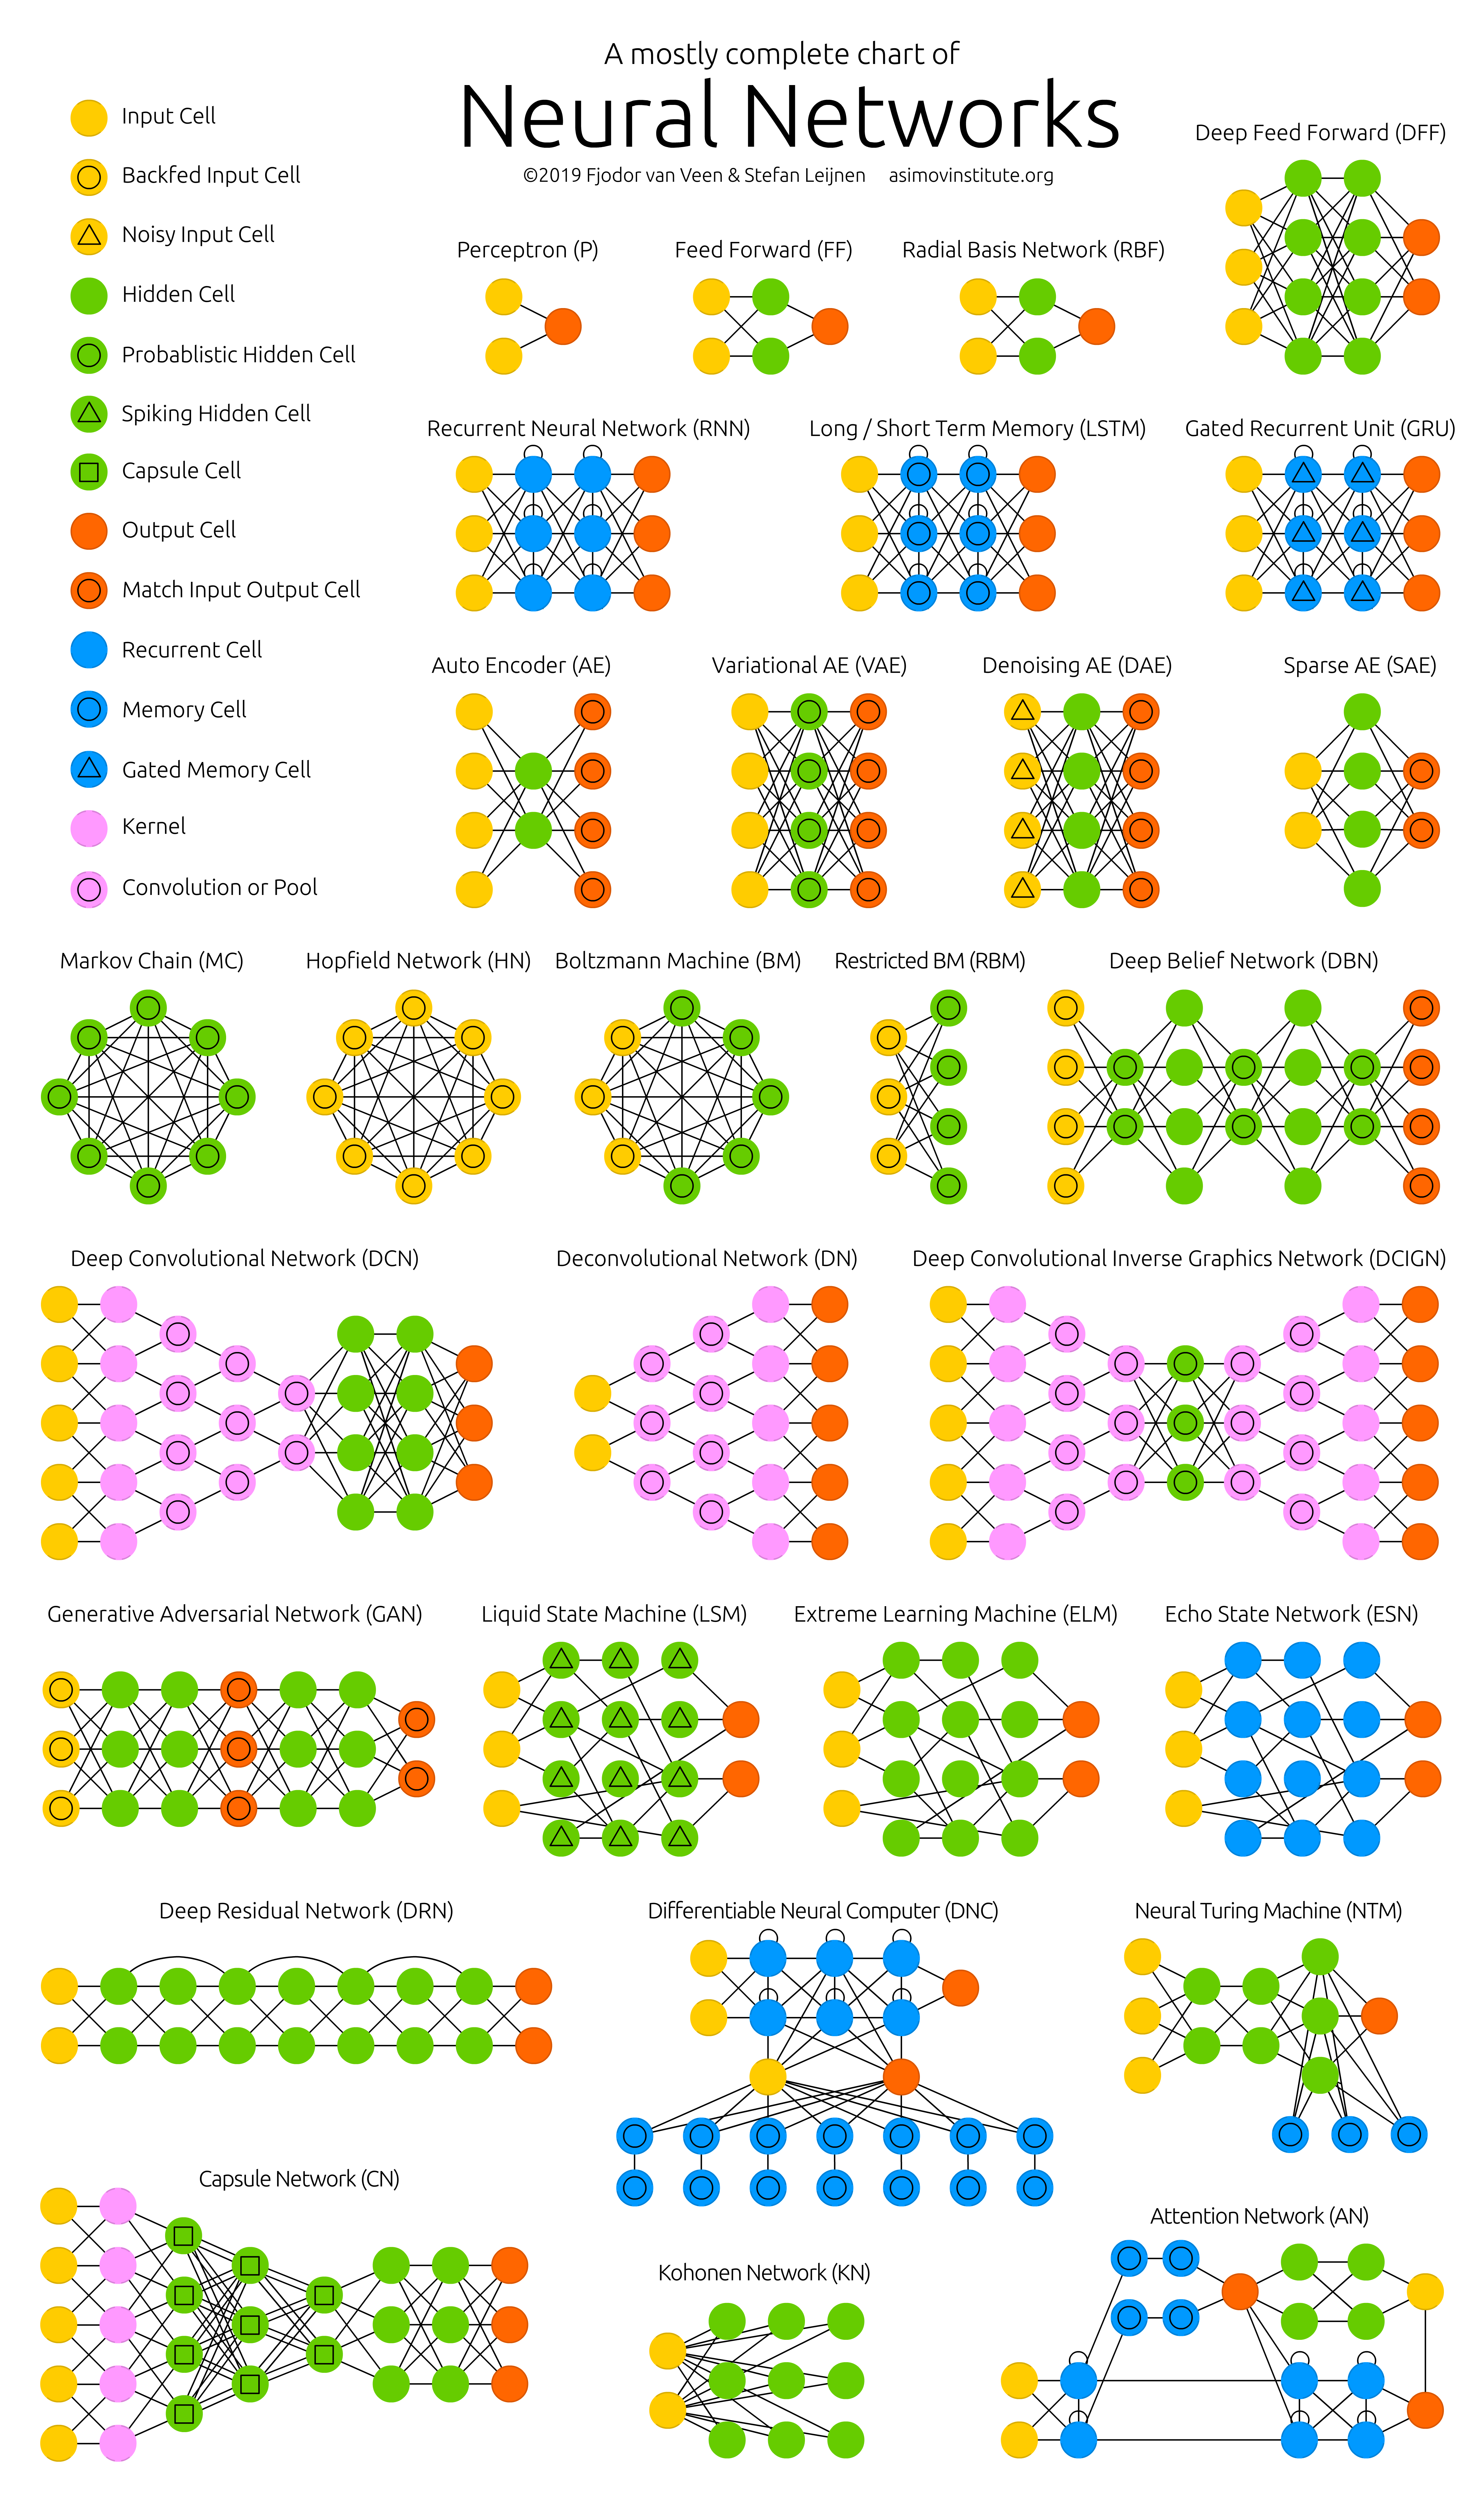
\includegraphics[totalheight=0.93\textheight]{graphics/NeuralNetworkZo19High}
\par\end{center}
\begin{itemize}
\item Universal Approximation Property--important for PINN and DeepONet
(see \textcolor{blue}{PINN Lecture})
\item Limits of universality:
\begin{itemize}
\item you may need to represent an exponentially complex network
\item if you can learn any function, then you WILL certainly \textcolor{magenta}{overfit}
\end{itemize}
\end{itemize}

\foilhead{NN - background and motivation}
\begin{itemize}
\item Previously (see above and in Basic Course), we discussed linear models
for regression and classification. 
\begin{itemize}
\item In particular, \textcolor{magenta}{logistic regression}, that in the
binary case, corresponds to the model 
\[
p(y|x,w)=\mathrm{Ber}(y|\sigma(w^{T}x)),
\]
\item \textcolor{magenta}{linear regression}, corresponds to the Gaussian
model 
\[
p(y|x,w)=\mathcal{N}(y|w^{T}x,\sigma^{2}).
\]
\item \textcolor{magenta}{generalized linear models} (GLM), that generalize
these models to other kinds of output distributions, such as Poisson. 
\item However, all these models make the strong assumption that the\textcolor{magenta}{{}
input-output mapping is linear.}
\end{itemize}
\item A simple way of increasing the flexibility of such models is to perform
a feature transformation, by replacing $x$ with $\varphi(x).$ 
\begin{itemize}
\item For example, we can use a polynomial transform, which in 1D is given
by $\varphi(x)=[1,x,x^{2},x^{3},...].$ This is sometimes called \textcolor{magenta}{basis
function expansion}. 
\item The model now becomes
\[
f(x;\theta)=W\varphi(x)+b
\]
\item This is still linear in the parameters $\theta=(W,b),$ which makes
model fitting easy (since the negative log-likelihood is convex).
However, having to specify the feature transformation by hand is very
limiting.
\end{itemize}
\item A natural extension is to endow the feature extractor with its own
parameters, $\theta_{2},$ to get
\[
f(x;\theta)=W\varphi(x;\theta_{2})+b
\]
where $\theta=(\theta_{1},\theta_{2})$and $\theta_{1}=(W,b).$ We
can obviously repeat this process recursively, to create more and
more complex functions. 
\item If we \textcolor{magenta}{compose} $L$ functions, we get
\[
f(x;\theta)=f_{L}(f_{L-1}(\cdot\cdot\cdot(f_{1}(x))\cdot\cdot\cdot))
\]
where $f_{l}(x)=f(x;\theta_{l})$ is the function at layer $l.$ This
is the key idea behind (deep) neural networks or (D)NNs.
\item The term \textquotedblleft (D)NN\textquotedblright{} actually encompasses
a larger family of models, in which we compose differentiable functions
into any kind of DAG (directed acyclic graph), mapping input to output.
\begin{itemize}
\item Equation above is the simplest example where the DAG is a chain. This
is known as a \textcolor{magenta}{feedforward neural network }(FFNN/FCNN)
or multilayer perceptron (MLP).
\item An MLP assumes that the input is a fixed-dimensional vector, say $x\in\mathbb{R}^{D}.$
\item It is common to call such data \textquotedblleft structured data\textquotedblright{}
or \textquotedblleft tabular data\textquotedblright , since the data
is often stored in an $N\times D$ \textcolor{magenta}{design matrix},
where each column (\textcolor{magenta}{feature}) has a specific meaning,
such as height, weight, age, etc. 
\end{itemize}
\item We discuss below other kinds of DNNs that are more suited to \textquotedblleft \textcolor{magenta}{unstructured
data}\textquotedblright{} such as images and text, where the input
data is variable sized, and each individual element (e.g., pixel or
word) is often meaningless on its own.
\begin{itemize}
\item \textcolor{magenta}{convolutional} neural networks (CNN), which are
designed to work with images; 
\item \textcolor{magenta}{recurrent} neural networks (RNN) and transformers,
which are designed to work with sequences
\item \textcolor{magenta}{graph} neural networks (GNN), which are designed
to work with graphs
\end{itemize}
\end{itemize}

\foilhead[-0.5in]{Neurons and Layers}

\begin{center}\index{neural networks (NN)!multi layer perceptron (MLP)|ffi}
\def\layersep{2.5cm}
\begin{tikzpicture}[shorten >=1pt,->,draw=black!50, node distance=\layersep]
\tikzstyle{every pin edge}=[<-,shorten <=1pt]
\tikzstyle{neuron}=[circle,fill=black!25,minimum size=17pt,inner sep=0pt]
\tikzstyle{input neuron}=[neuron, fill=green!50];
\tikzstyle{output neuron}=[neuron, fill=red!50];
\tikzstyle{hidden neuron}=[neuron, fill=blue!50];
\tikzstyle{annot} = [text width=4em, text centered]

% Draw the input layer nodes
\foreach \name / \y in {1,...,4}
% This is the same as writing \foreach \name / \y in {1/1,2/2,3/3,4/4}
\node[input neuron, pin=left:Input $x_{\y}$] (I-\name) at (0,-\y) {};

% Draw the hidden layer nodes
\foreach \name / \y in {1,...,5}
\path[yshift=0.5cm]
node[hidden neuron] (H-\name) at (\layersep,-\y cm) {};

% Draw the output layer node
\node[output neuron,pin={[pin edge={->}]right:Output $y$}, right of=H-3] (O) {};

% Connect every node in the input layer with every node in the
% hidden layer.
\foreach \source in {1,...,4}
\foreach \dest in {1,...,5}
\path (I-\source) edge (H-\dest);

% Connect every node in the hidden layer with the output layer
\foreach \source in {1,...,5}
\path (H-\source) edge (O);

% Annotate the layers
\node[annot,above of=H-1, node distance=2cm] (hl) {Hidden layer};
\node[annot,left of=hl] {Input layer};
\node[annot,right of=hl] {Output layer};
\end{tikzpicture}
\end{center}

\begin{figure}
\begin{centering}
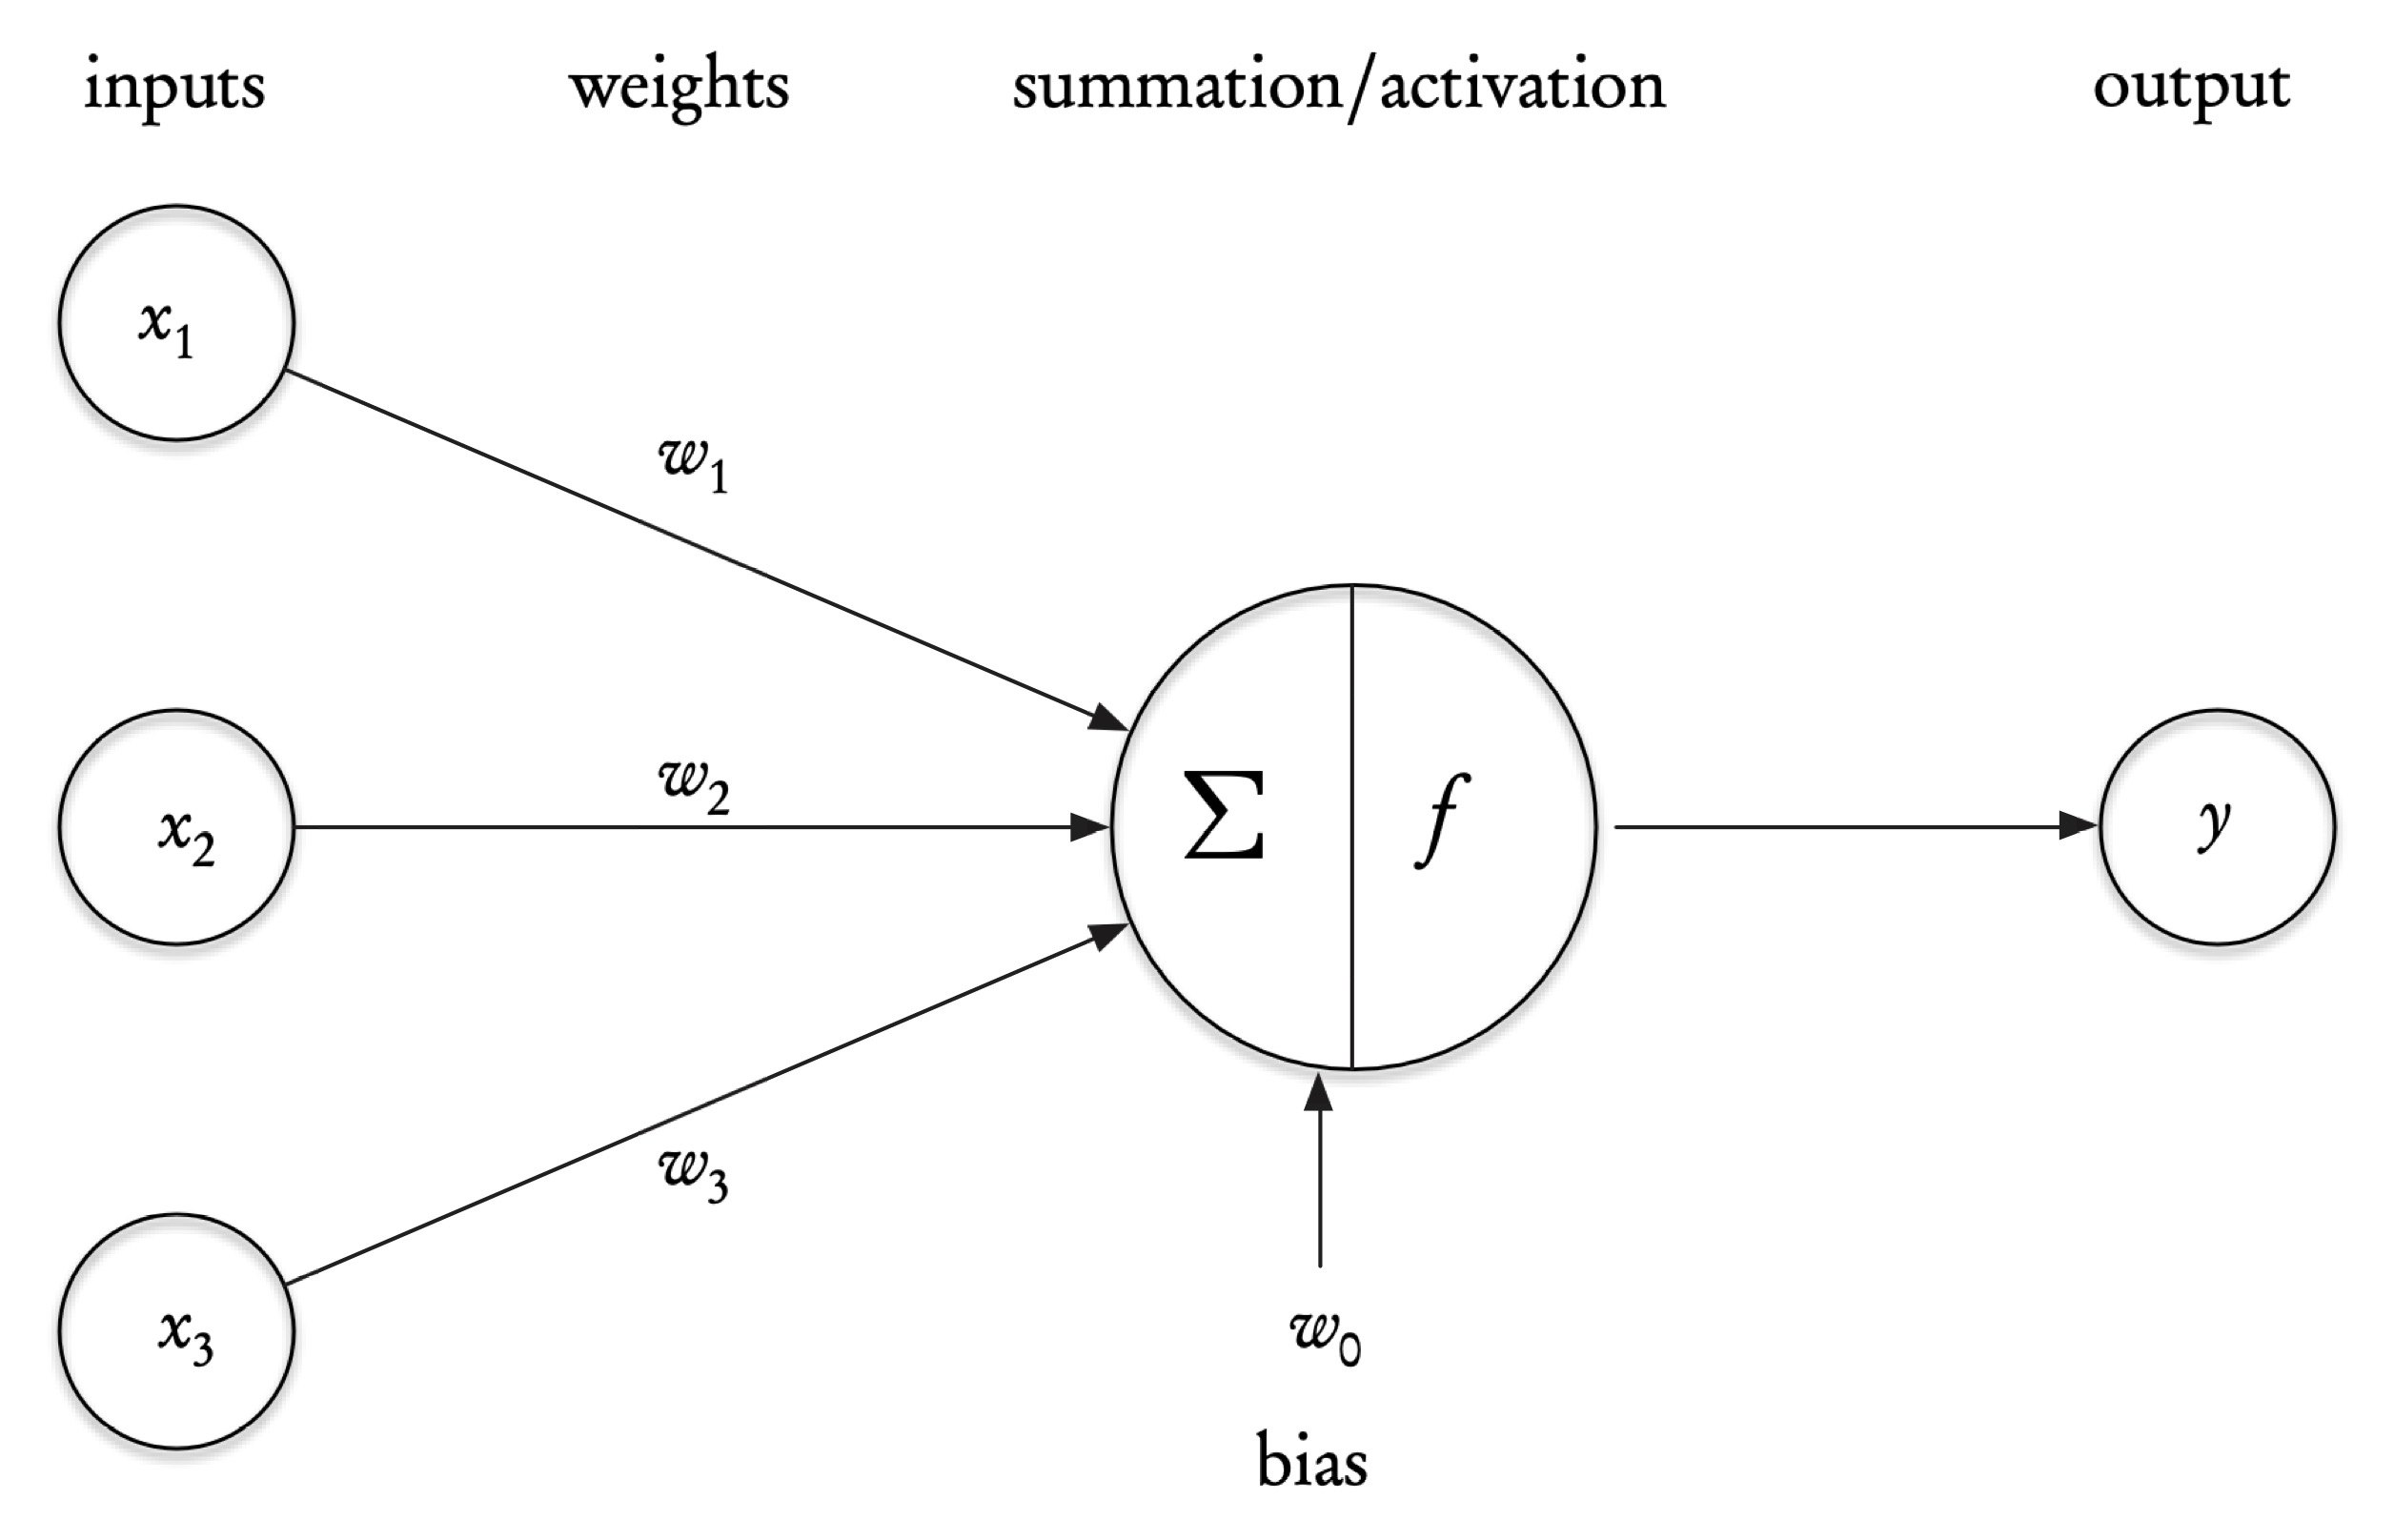
\includegraphics[scale=0.5]{/Users/markasch/Dropbox/6Books/DTbook/src/bwgraphics/neuron}
\par\end{centering}
\caption{A single neuron with output $y=f\left(w_{0}+\sum_{i=1}^{3}w_{i}x_{i}\right)$}
\end{figure}


\foilhead{Differentiable MLPs}
\begin{itemize}
\item For MLPs, we define differentiable activation functions $\varphi:\mathbb{R}\rightarrow R.$
More precisely, we define the hidden units $z_{l}$ at each layer
$l$ to be a linear transformation of the hidden units at the previous
layer passed element-wise through this activation function,
\[
z_{l}=f_{l}(z_{l-1})=\varphi_{l}(b_{l}+W_{l}z_{l-1})
\]
\item If we now compose $L$ of these functions together, we can compute
the \textcolor{magenta}{gradient} of the output with respect to the
parameters in each layer using the \textcolor{magenta}{chain rule},
also known as \textcolor{magenta}{backpropagation}, as we explain
in the Lecture on \textcolor{blue}{Automatic Differentiation}.
\item And once we have the gradient, we can invoke a \textcolor{magenta}{gradient-based
optimization} algorithm to minimize a loss function, measuring the
mismatch between the model and the measurements, as usual.
\end{itemize}

\foilhead{Activation Functions}
\begin{itemize}
\item In the early days of neural networks, a common choice was to use a
\textcolor{magenta}{sigmoid} (logistic) function, which can be seen
as a smooth approximation to the Heaviside function used in a perceptron
\[
\sigma(a)=\frac{1}{1+\mathrm{e}^{-a}}
\]
\item However, the sigmoid function \textcolor{magenta}{saturates} at $1$
for large positive inputs, and at $0$ for large negative inputs. 
\item Another common choice is the \textcolor{magenta}{tanh }function, which
has a similar shape, but saturates at $-1$ and $+1.$
\item In the saturated regimes, the gradient of the output wrt the input
will be close to zero, so any gradient signal from higher layers will
not be able to propagate back to earlier layers. This is called the
\textcolor{magenta}{vanishing gradient} problem, and it makes it hard
to train the model using gradient descent.
\item One of the keys to being able to train very deep models is to use
\textcolor{magenta}{non-saturating} activation functions. Several
different functions have been proposed. The most common is rectified
linear unit or ReLU, 
\[
\mathrm{ReLU}(a)=\max(a,0)=a\mathbb{I},\quad(a>0)
\]
\item All of the above, together with the availability of data, open-source
software and GPU accelerators, has led to the ``\textcolor{red}{deep
learning revolution}'' that started in the 2010's (about a decade
ago...)
\end{itemize}
\begin{center}
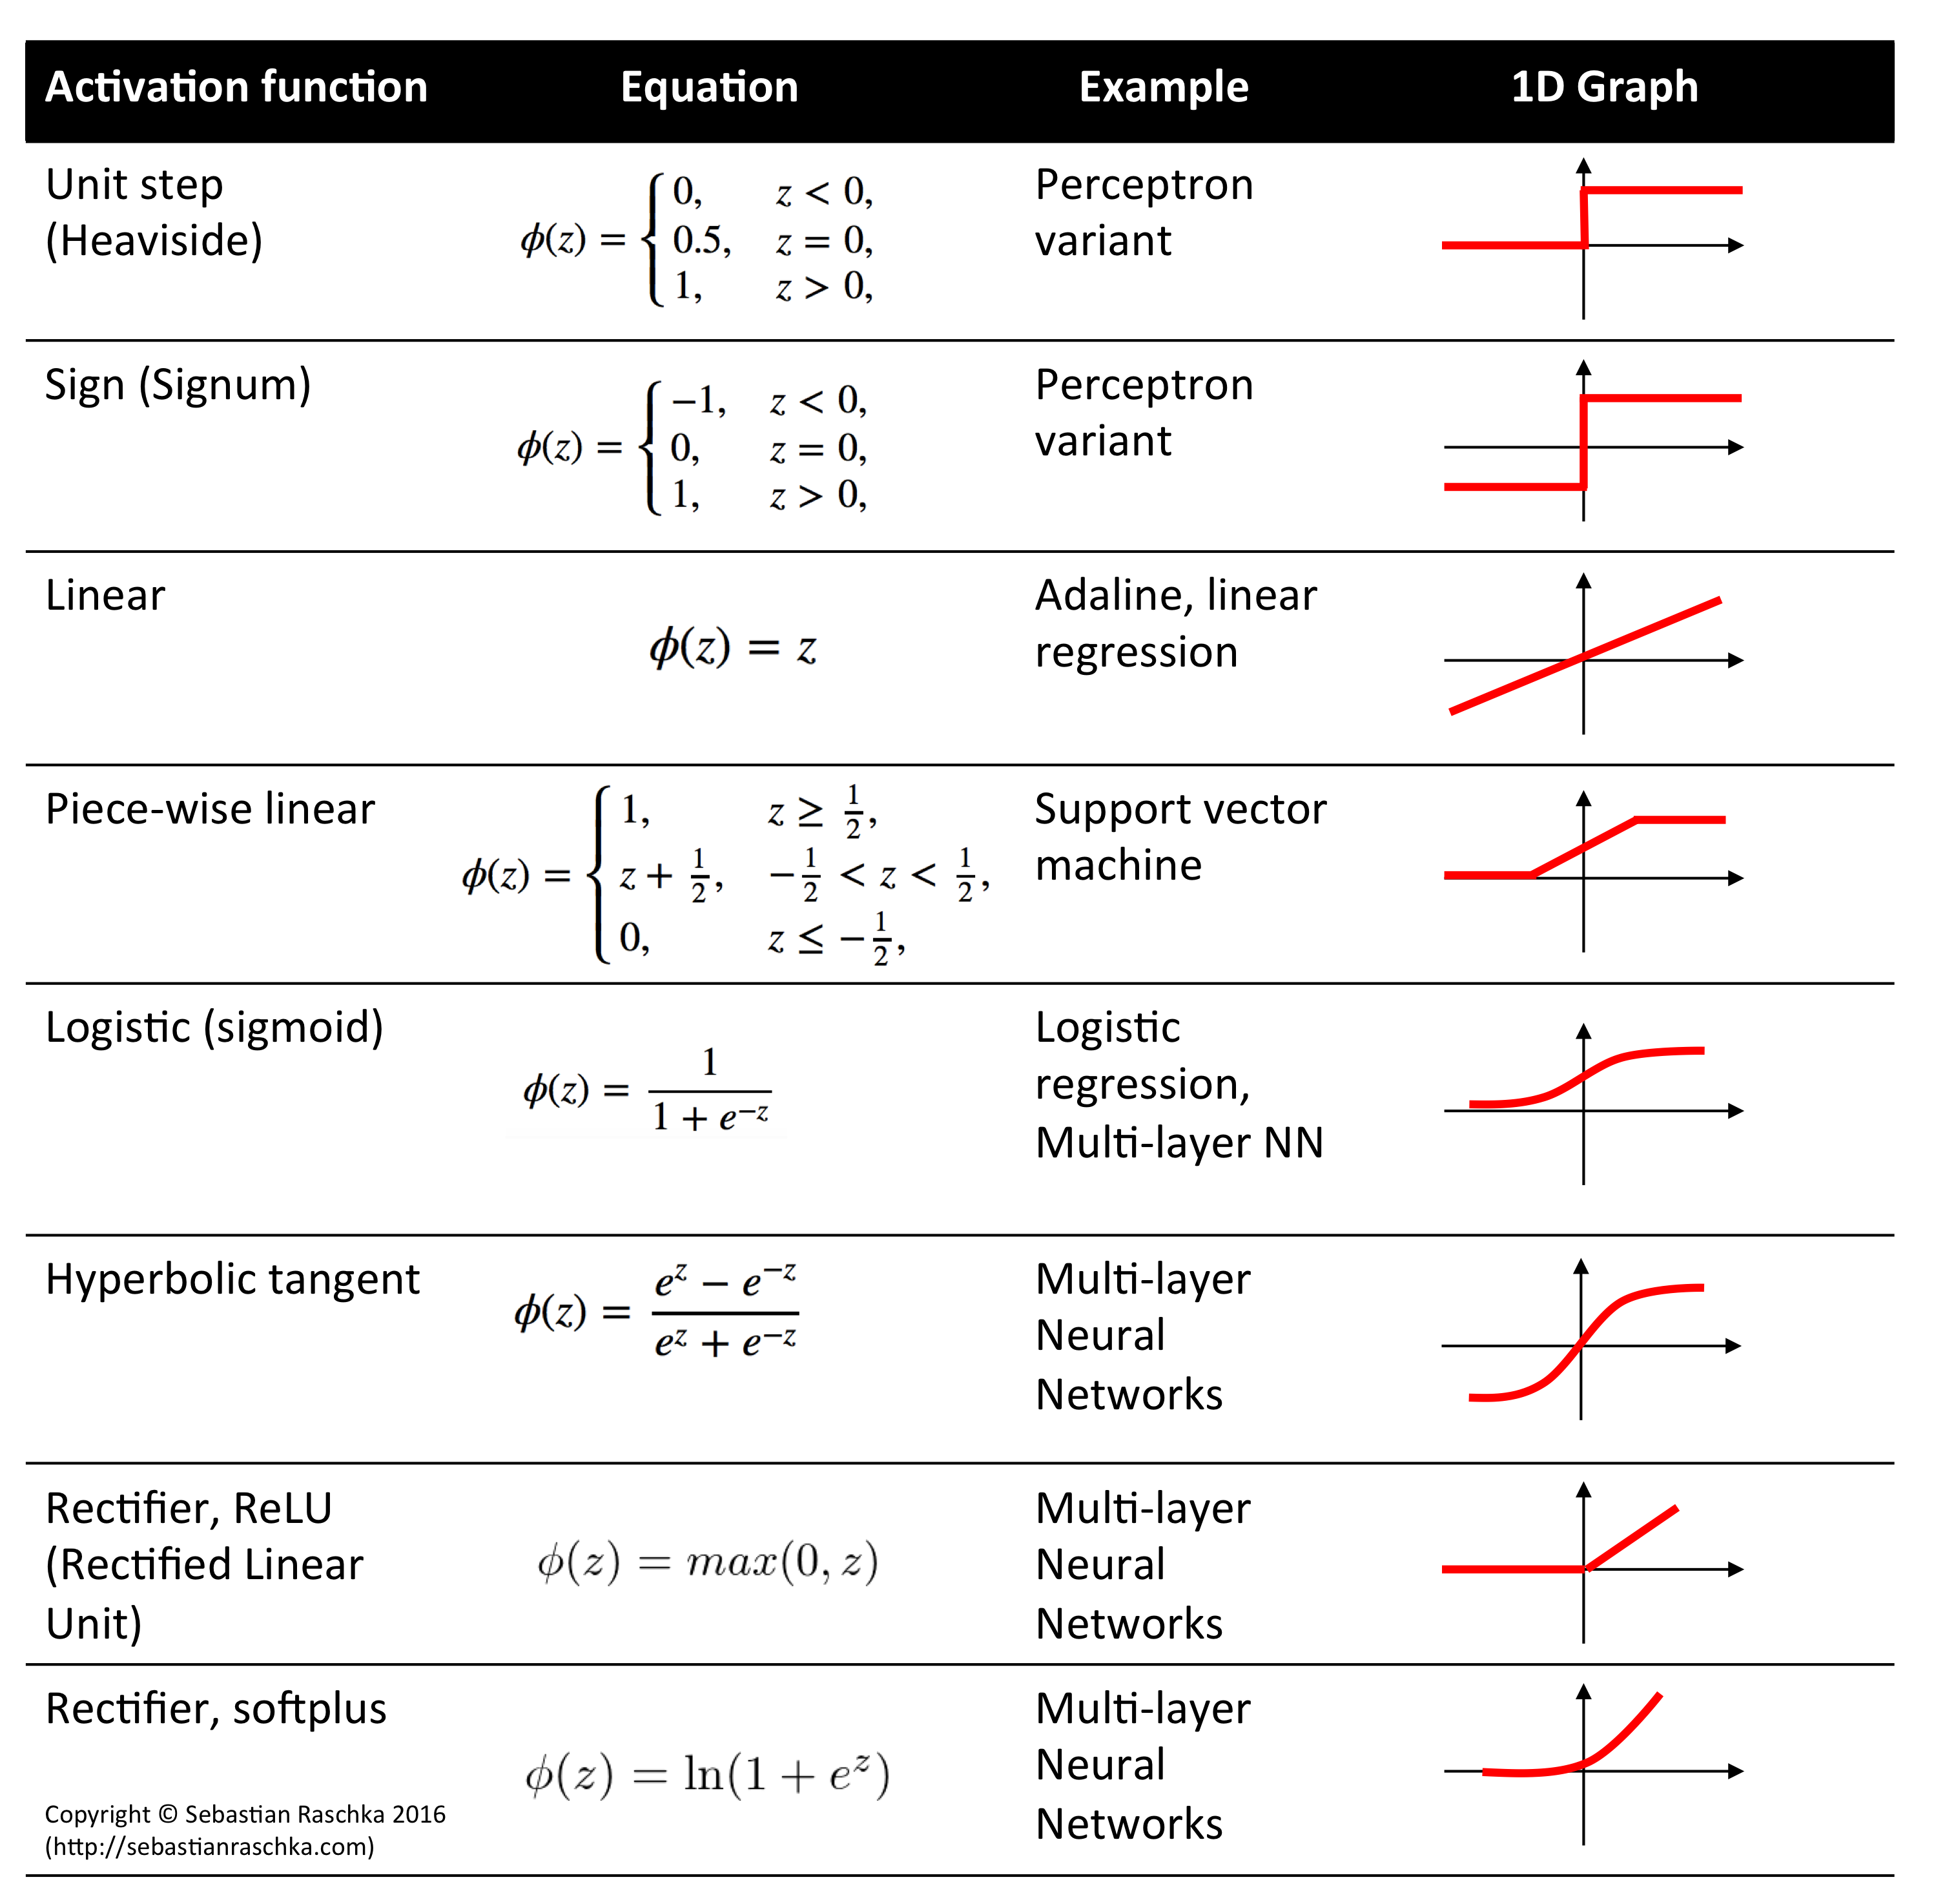
\includegraphics[totalheight=0.9\textheight]{graphics/activation-functions}
\par\end{center}

\foilhead{Choice of Activation for Output Layer}
\begin{itemize}
\item The use of sigmoid activation functions in a neural network doesn't
necessarily restrict the output values to the interval {[}0, 1{]}.
However, it's important to understand when and why the sigmoid activation
may or may not constrain the output.
\item 1. {*}{*}Sigmoid's Range{*}{*}: The sigmoid activation function has
a mathematical form that maps any real number to a value between 0
and 1. Specifically, the sigmoid function is defined as:
\[
\sigma(x)=\frac{1}{1+e^{-x}}
\]
This function \textquotedbl squashes\textquotedbl{} its input into
the {[}0, 1{]} range, and it's often used in the context of binary
classification problems where the output can be interpreted as a probability.
\item 2. {*}{*}Sigmoid as Hidden Activation{*}{*}: When you use sigmoid
activations in hidden layers of a neural network, they introduce non-linearity
and can help the network learn complex patterns. These sigmoid activations
do not constrain the output to the {[}0, 1{]} range. The output is
influenced by the combination of activations and weights in subsequent
layers.
\item 3. {*}{*}Output Layer Activation{*}{*}: If you use sigmoid as the
activation function in the output layer, it implies that the network
is designed for binary classification, and the output is expected
to represent probabilities. In this case, the output will be in the
{[}0, 1{]} range.
\item 4. {*}{*}Other Output Activations{*}{*}: To have a network with output
values outside the {[}0, 1{]} range, you should use different activation
functions in the output layer. Common choices include linear (no activation)
for regression problems or other activation functions like softmax
for multi-class classification.
\end{itemize}
In summary, the use of sigmoid activations in hidden layers contributes
to the network's capacity to model complex functions but does not
inherently restrict the output to the {[}0, 1{]} range. The final
output's range depends on the activation function used in the output
layer, and you have flexibility in choosing an appropriate activation
based on your specific problem.

\foilhead{Universal Approximation Theory---the secret of SUCCESS}
\begin{thm}
[Cybenko 1989]If $\sigma$ is any continuous sigmoidal function,
then finite sums 
\[
G(x)=\sum_{j=1}^{N}\alpha_{j}\sigma\left(y_{j}\cdot x+\theta_{j}\right)
\]
 are dense in $C(I_{d}).$
\end{thm}
%
\vspace{.5\baselineskip}

\vspace{.5\baselineskip}

\begin{thm}
[Pinkus 1999]Let $\mathbf{m}_{i}\in\mathbb{Z}^{d},$ $i=1,\ldots,s,$
and set $m=\max_{i}\left|\mathbf{m}^{i}\right|.$ Suppose that $\sigma\in C^{m}(\mathbb{R}),$
not polynomial. Then the space of \textcolor{red}{single hidden layer}
neural nets, 
\[
\mathcal{M}(\sigma)=\mathrm{span}\left\{ \sigma(\mathbf{w}\cdot\mathbf{x}+b)\colon\mathbf{w}\in\mathbb{R}^{d},\,b\in\mathbb{R}\right\} ,
\]
is dense in $C^{\mathbf{m}^{1},\ldots,\mathbf{m}^{s}}(\mathbb{R}^{d})\doteq\cap_{i=1}^{s}C^{\mathbf{m}^{i}}(\mathbb{R}^{d}).$
\end{thm}

\foilhead{NNs and AI - connections with biology?}
\begin{center}
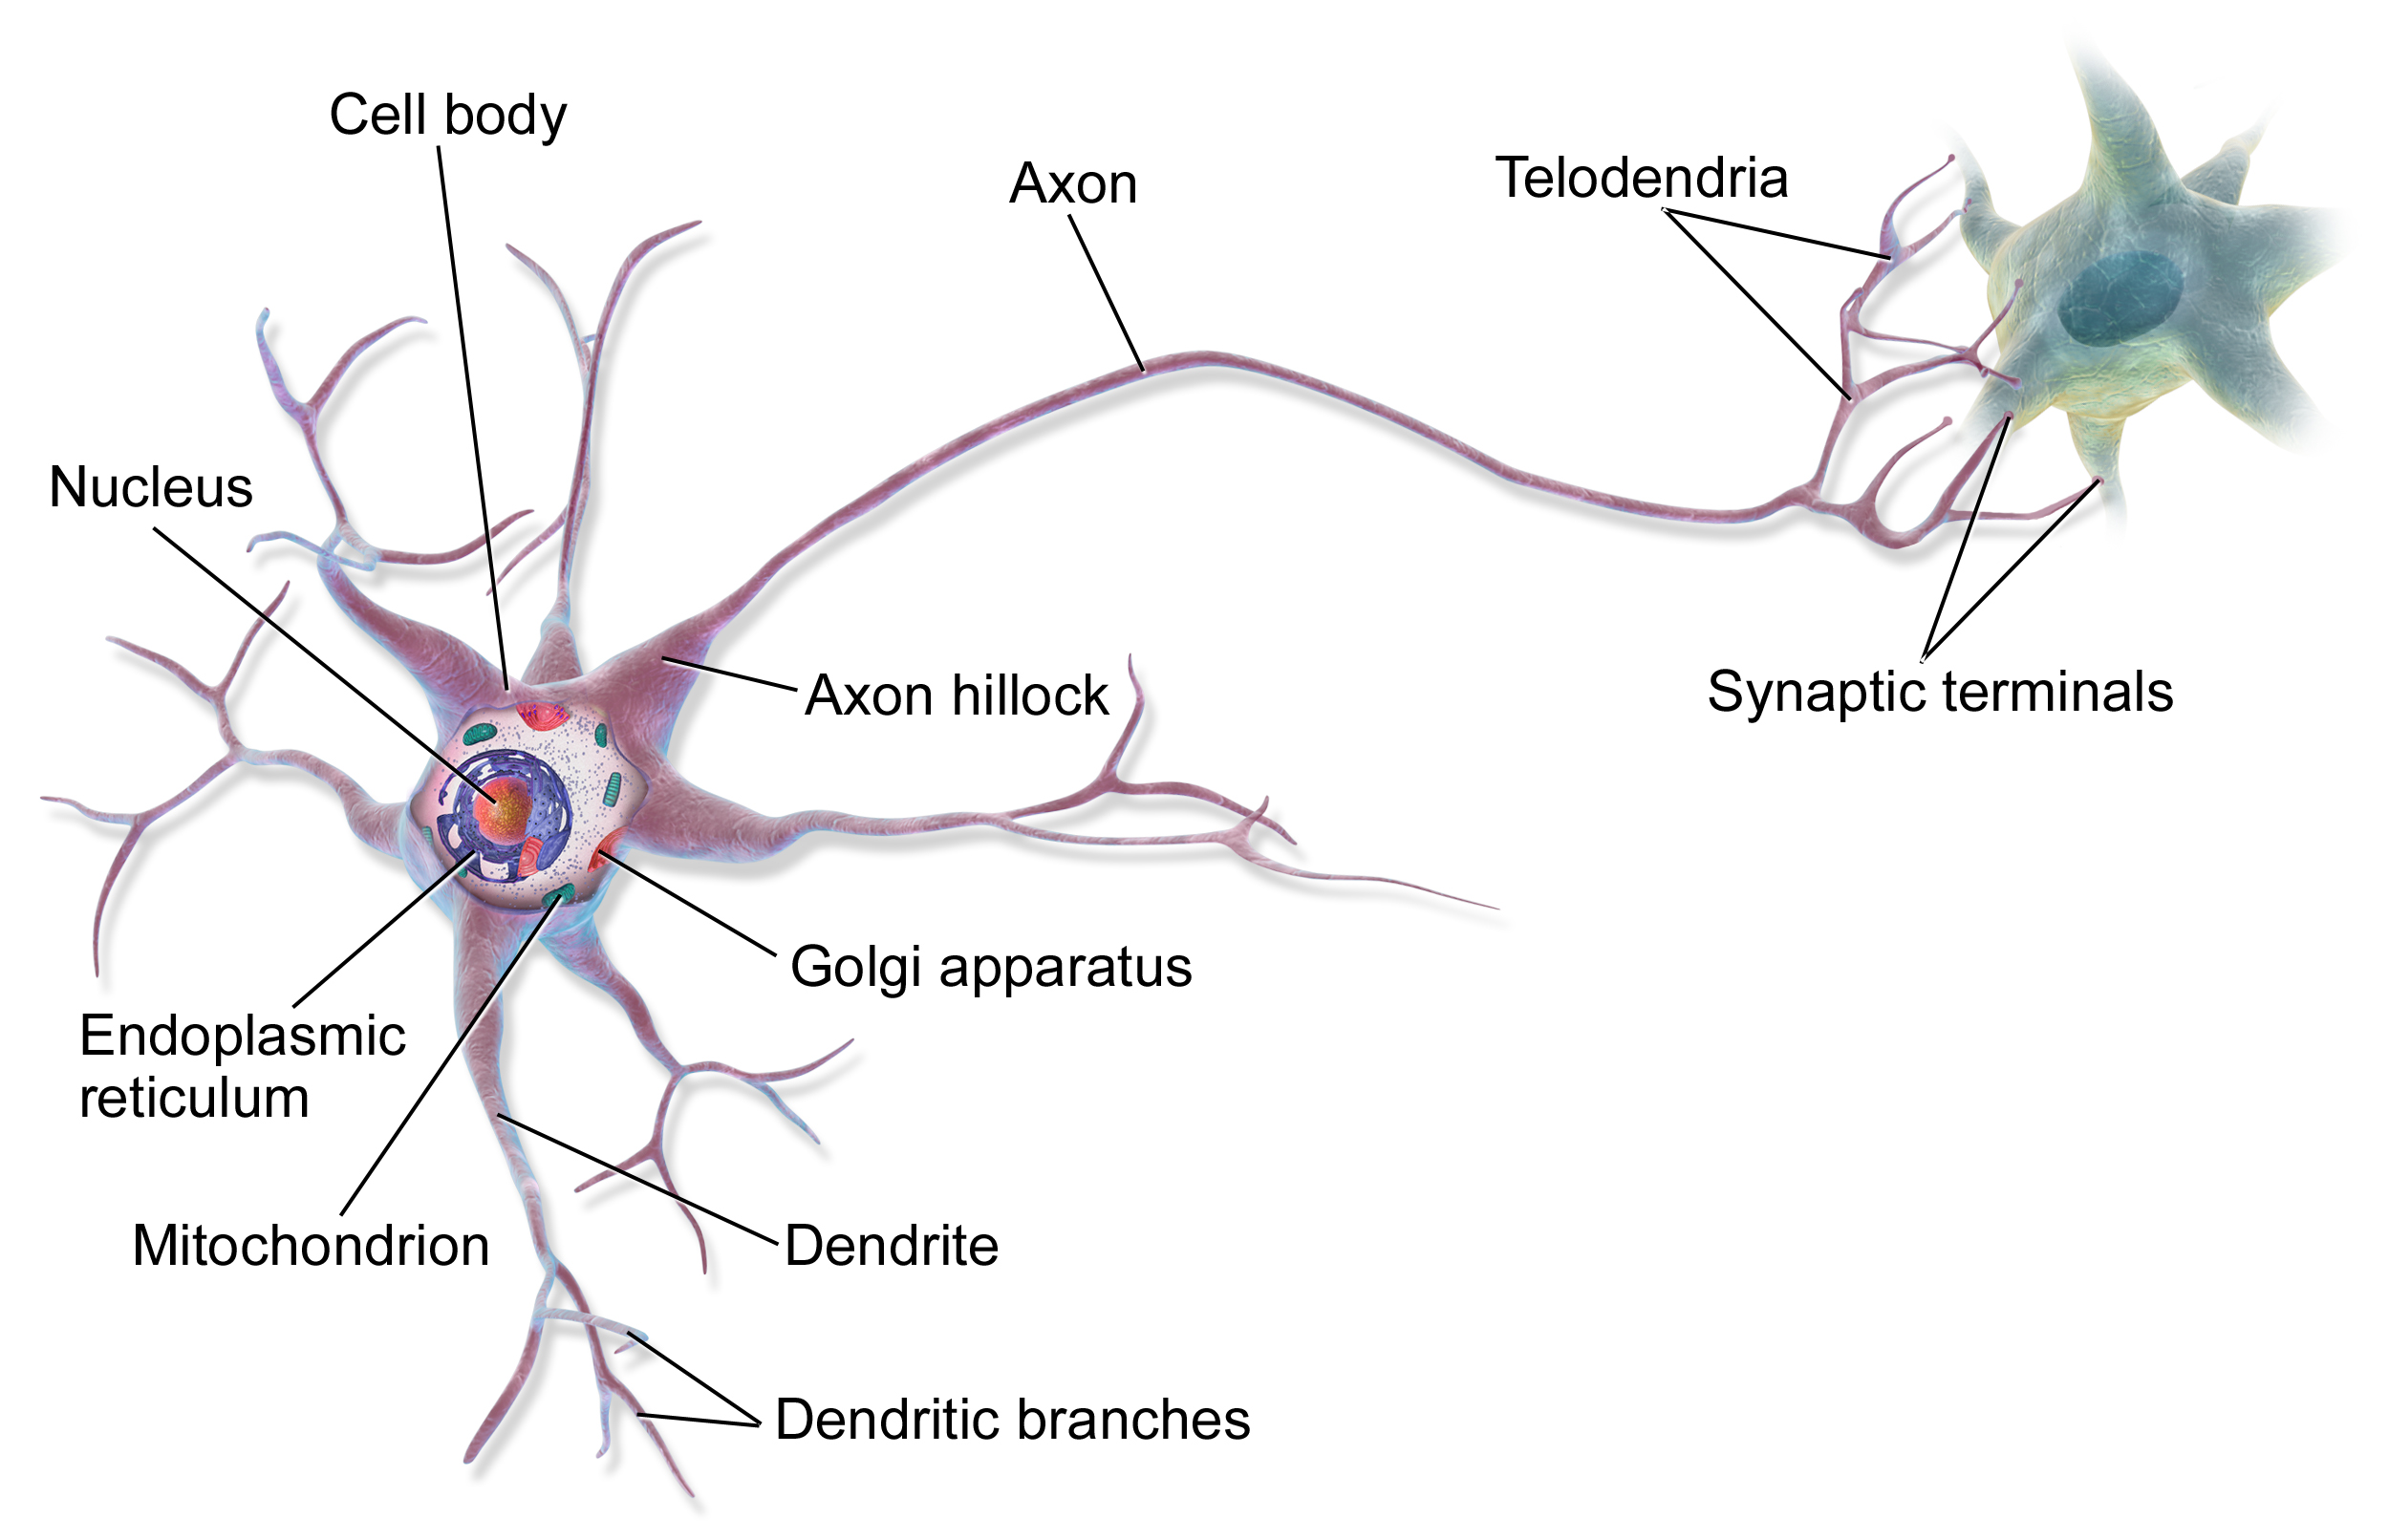
\includegraphics[width=0.8\textheight]{graphics/axon}
\par\end{center}
\begin{itemize}
\item What are the connections between the kinds of neural networks we have
discussed above, known as \textcolor{magenta}{artificial neural networks}
or ANNs, and \textcolor{magenta}{real} neural networks, as found in
humans and in the animal kingdom?
\item Let us consider a model of a \textcolor{magenta}{single neuron}...
\begin{itemize}
\item To a first approximation, we can say that whether neuron $k$ fires,
denoted by $h_{k}\in\left\{ 0,1\right\} ,$ depends on the activity
of its inputs, denoted by $x\in\mathbb{R}^{D},$ as well as the strength
of the incoming connections, which we denote by $w_{k}\in\mathbb{R}^{D}.$ 
\item We can compute a weighted sum of the inputs using $a_{k}=w_{k}^{T}x.$
These weights can be viewed as \textquotedblleft wires\textquotedblright{}
connecting the inputs $x_{d}$ to neuron $h_{k};$ these are analogous
to dendrites in a real neuron.
\item This weighted sum is then compared to a threshold, $b_{k},$ and if
the activation exceeds the threshold, the neuron fires; this is analogous
to the neuron emitting an electrical output or action potential. 
\item Thus we can model the behavior of the neuron using $h_{k}(x)=H(w_{k}^{T}x-b_{k}),$
where $H(a)=\mathbb{I}(a>0)$ is the Heaviside function. This is called
the McCulloch-Pitts model of the neuron, and was proposed in 1943...
\end{itemize}
\item We can then combine multiple such neurons together to make an ANN.
The result has sometimes been viewed as a model of the brain. 
\item However, \textcolor{magenta}{ANNs differ from biological brains }in
many ways, including the following:
\begin{itemize}
\item Most ANNs use \textcolor{magenta}{backpropagation} to modify the strength
of their connection. However, real brains do not use backprop, since
there is no way to send information backwards along an axon. Instead,
they use local update rules for adjusting synaptic strengths.
\item Most ANNs are strictly \textcolor{magenta}{feedforward}, but real
brains have many feedback connections. It is believed that this feedback
acts like a prior, which can be combined with bottom up likelihoods
from the sensory system to compute a posterior over hidden states
of the world, which can then be used for optimal decision making.
\item Most ANNs use \textcolor{magenta}{simplified} neurons consisting of
a weighted sum passed through a nonlinearity, but real biological
neurons have complex dendritic tree structures (see Figure), with
complex spatio-temporal dynamics.
\item Most ANNs are \textcolor{magenta}{smaller} in size and number of connections
than biological brains. Of course, ANNs are getting larger every week,
fueled by various new hardware accelerators, such as GPUs and TPUs
(tensor processing units), etc. However, even if ANNs match biological
brains in terms of number of units, the comparison is misleading since
the processing capability of a biological neuron is much higher than
an artificial neuron (see point above).
\item Most ANNs are designed to model a \textcolor{magenta}{single} function,
such as mapping an image to a label, or a sequence of words to another
sequence of words. By contrast, biological brains are very complex
systems, composed of multiple specialized interacting modules, which
implement different kinds of functions or behaviors such as perception,
control, memory, language, etc.
\end{itemize}
\item It is commonly believed that the\textcolor{magenta}{{} low level details}
of biological brains do not matter if our goal is to build \textquotedblleft intelligent
machines\textquotedblright , just as aeroplanes do not flap their
wings. However, presumably \textquotedblleft AIs\textquotedblright{}
will follow similar \textquotedblleft laws of intelligence\textquotedblright{}
to intelligent biological agents, just as planes and birds follow
the same laws of aerodynamics.
\item Unfortunately, we do not yet know what the \textquotedblleft \textcolor{magenta}{laws
of intelligence}\textquotedblright{} are, or indeed if there even
are such laws. One approach is to make the assumption that any intelligent
agent should follow the basic principles of information processing
and \textcolor{magenta}{Bayesian decision theory}, which is known
to be the optimal way to make decisions under uncertainty.
\item In practice, the optimal Bayesian approach is often \textcolor{magenta}{computationally
intractable}. In the natural world, biological agents have evolved
various algorithmic \textquotedblleft shortcuts\textquotedblright{}
to the optimal solution; this can explain many of the heuristics that
people use in everyday reasoning. As the tasks we want our machines
to solve become harder, we may be able to gain insights from \textcolor{magenta}{neuroscience}
and cognitive science for how to solve such tasks in an approximate
way. However, we should also bear in mind that AI/ML systems are increasingly
used for \textcolor{magenta}{safety-critical} applications, in which
we might want and expect the machine to do better than a human. In
such cases, we may want more than just heuristic solutions that often
work; instead we may want provably reliable methods, similar to other
engineering fields... There is still a long way to go before reaching
this point---see \textcolor{blue}{Bias and Ethics Lectures}. 
\end{itemize}

\foilhead{$\;$}

\vfill{}

\begin{center}
{\Large\textbf{\textcolor{blue}{UNSUPERVISED LEARNING}}}{\Large\par}
\par\end{center}

\vfill{}


\foilhead{Clustering}
\begin{itemize}
\item Evaluating clustering results is inevitably subjective. For supervised
classification, we have the true labels. Therefore, we can compute
the error rate to assess the result. However, in \textcolor{magenta}{unsupervised}
clustering, we do not have the class labels given for the training
data.
\begin{itemize}
\item One \textcolor{magenta}{heuristic} generally accepted is that points
in the same cluster should be tight and points in different groups
should be as far apart as possible. 
\end{itemize}
\item \textcolor{magenta}{$k$-means}: 
\begin{itemize}
\item The k-means algorithm reflects the heuristic by attempting to minimize
the total \textcolor{magenta}{within-cluster} distances between each
data point and its corresponding prototype (or centroid).
\end{itemize}
\item The\textcolor{magenta}{{} agglomerative clustering} method is also called
a bottom-up method as opposed to k-means or k-center methods that
are top-down. 
\begin{itemize}
\item In a top-down method, a data set is divided into more and more clusters. 
\item In a bottom-up approach, all the data points are treated as individual
clusters to start with and gradually merged into bigger and bigger
clusters.
\end{itemize}
\item In agglomerative clustering, clusters are generated \textcolor{magenta}{hierarchically}. 
\begin{itemize}
\item We start by taking every data point as a cluster. 
\item Then we merge two clusters at a time. 
\item In order to decide which two clusters to merge, we compare the pairwise
distances between any two clusters and pick a pair with the minimum
distance. Once we merge two clusters into a bigger one, a new cluster
is created. 
\item The distances between this new cluster and the existing ones are not
given. Some scheme has to be used to obtain these distances based
on the two merged clusters. We call this the update of distances.
Various schemes of updating distances will be described shortly.
\end{itemize}
\item We can keep merging clusters until all the points are merged into
one cluster. A tree can be used to visualize the merging process.
This tree is called a \textcolor{magenta}{dendrogram}.
\item How do we get the distance between the new cluster and the existing
clusters?
\begin{itemize}
\item The idea is to somehow aggregate the distances between the objects
contained in the clusters.
\begin{itemize}
\item For clusters containing only one data point, the between-cluster distance
is the between-object distance.
\item For clusters containing multiple data points, the between-cluster
distance is an agglomerative version of the between-object distances.
There are a number of ways to accomplish this. Examples of these aggregated
distances include the \textcolor{magenta}{minimum} , \textcolor{magenta}{average}
or \textcolor{magenta}{maximum} between-object distances for pairs
of objects across the two clusters.
\item Possibilities are: Single-link clustering (minimum distance), Complete-link
clustering (maximum distance), Average linkage clustering, Centroid
clustering and Ward's clustering.
\end{itemize}
\end{itemize}
\item How do we decide which aggregation scheme to use? 
\begin{itemize}
\item Depending on how we update the distances, dramatically different results
may come up. 
\item Therefore, it is always good practice to look at the results using
scatterplots or other visualization methods instead of blindly taking
the output of any algorithm. 
\item Clustering is inevitably \textcolor{magenta}{subjective} since there
is no gold standard.
\end{itemize}
\end{itemize}

\foilhead{PCA}
\begin{itemize}
\item Principal Component Analysis (PCA) is a method of \textcolor{magenta}{dimension
reduction}. 
\item This is not directly related to prediction problems, but 
\begin{itemize}
\item several regression methods are directly dependant on it, such as PCR
and PLS, and
\item it can be used as a part of EDA (exploratory data analysis)
\end{itemize}
\item PCA uses the \textcolor{magenta}{eigendecomposition} of the \textcolor{magenta}{covariance}
matrix, $\mathbf{\Sigma}=\mathbf{X}^{T}\mathbf{X},$ based on an SVD
algorithm.
\item Recall: The first principal component direction $\mathbf{v}_{1}$
has the following properties
\begin{itemize}
\item $\mathbf{v}_{1}$ is the eigenvector associated with the largest eigenvalue
$\sigma_{1}^{2}$ of $\mathbf{X}^{T}\mathbf{X}$
\item $\mathbf{z}_{1}=\mathbf{X}\mathbf{v}_{1}$ has the \textcolor{magenta}{largest
sample variance} amongst all normalized linear combinations of the
columns of $\mathbf{X}.$
\item $\mathbf{z}_{1}$ is called the first principal component of $\mathbf{X}$
and we have $\Var(\mathbf{z}_{1})=\sigma_{1}^{2}/N.$ The second principal
component direction $\mathbf{v}_{2}$ (the direction orthogonal to
the first component that has the largest projected variance) is the
eigenvector corresponding to the second largest eigenvalue, etc.
\end{itemize}
\item The \textcolor{magenta}{variance} of the data along the principal
component directions is associated with the magnitude of the eigenvalues.
\end{itemize}

\foilhead{$\;$}

\vfill{}

\begin{center}
{\Large\textbf{\textcolor{blue}{DEEP Neural Networks}}}{\Large\par}
\par\end{center}

\vfill{}


\foilhead{Overview of DNNs}
\begin{itemize}
\item As seen above in the NN ``zoo'', there is an increasingly large number
and diversity of neural networks
\end{itemize}
\begin{defn}
A \textcolor{magenta}{deep neural network} is a neural network with
a level of complexity beyond that of a simple feedforward network.
Deep neural networks use sophisticated mathematical modeling to process
data in complex ways. The adjective \textquotedbl deep\textquotedbl{}
in deep learning refers to the use of multiple layers in the network.
Methods used can be either supervised, semi-supervised or unsupervised.
\end{defn}
\begin{itemize}
\item Here is an annotated list of some of the more common DNNs, with their
application domains.
\end{itemize}
\begin{center}
{\small{}%
\begin{tabular}{|c|c|}
\hline 
{\small DNN Type} & {\small Applications}\tabularnewline
\hline 
\hline 
{\small Convolutional-CNN} & \begin{cellvarwidth}[t]
\centering
{\small Image processing, object detection, }\\
{\small natural language processing}
\end{cellvarwidth}\tabularnewline
\hline 
{\small Recurrent-RNN} & \begin{cellvarwidth}[t]
\centering
{\small Time series, natural language processing, }\\
{\small speech recognition, machine translation}
\end{cellvarwidth}\tabularnewline
\hline 
{\small LSTM, GRU} & {\small Variants of RNN}\tabularnewline
\hline 
{\small Autoencoder} & \begin{cellvarwidth}[t]
\centering
{\small Noise filtering, Dimensionality reduction, }\\
{\small image compression, anomaly detection}
\end{cellvarwidth}\tabularnewline
\hline 
{\small Adversarial-GAN} & \begin{cellvarwidth}[t]
\centering
{\small AlphaGo, Image generation, text generation, }\\
{\small music generation}
\end{cellvarwidth}\tabularnewline
\hline 
{\small Graph-GNN } & \begin{cellvarwidth}[t]
\centering
{\small image classification, image recognition, }\\
{\small object detection}
\end{cellvarwidth}\tabularnewline
\hline 
{\small Transformer-GPT} & {\small Natural language processing, machine translation}\tabularnewline
\hline 
\end{tabular}}{\small\par}
\par\end{center}
\begin{itemize}
\item \textbf{Multilayer perceptron (MLP)} is the simplest type of deep
neural network. It is a feedforward network, which means that the
data flows in one direction from the input layer to the output layer.
MLPs are often used for classification tasks, such as image classification
and natural language processing.
\item \textbf{Convolutional neural network (CNN) }is a type of DNN that
is specifically designed for processing images. CNNs use convolution
operations to extract features from images. They are often used for
image classification, object detection, and natural language processing
tasks that involve images.
\item \textbf{Recurrent neural network (RNN)} is a type of DNN that is specifically
designed for processing sequences of data. RNNs use recurrence connections
to allow them to remember the past inputs. They are often used for
natural language processing tasks, such as speech recognition and
machine translation.
\item \textbf{Long short-term memory network (LSTM)} is a type of RNN that
is specifically designed to handle long-term dependencies. LSTMs use
gates to control the flow of information through the network, which
allows them to learn long-term patterns in data. They are often used
for natural language processing tasks that require long-term memory,
such as machine translation.
\item \textbf{Autoencoder} is a type of neural network that can be used
to compress data or to extract features from data. It consists of
two parts, an encoder and a decoder. The encoder compresses the data
into a latent representation, while the decoder reconstructs the data
from the latent representation.
\item \textbf{Generative adversarial network (GAN)} is a type of DNN that
is used to generate new data. GANs consist of two networks, a generator
and a discriminator. The generator is responsible for creating new
data, while the discriminator is responsible for distinguishing between
real and fake data. GANs are often used for image generation, text
generation, and music generation.
\item \textbf{Deep reinforcement learning (DRL) }is a type of machine learning
that uses DNNs to learn how to behave in an environment. DRL agents
learn by trial and error, and they are often used for robotics and
game playing.
\item \textbf{Graph Neural Networks (GNNs)} are a class of deep learning
methods designed to perform inference on data described by graphs.
GNNs are neural networks that can be directly applied to graphs, and
provide an easy way to do node-level, edge-level, and graph-level
prediction tasks.
\item \textbf{Transformer }is a type of DNN that is specifically designed
for natural language processing tasks. Transformers use attention
mechanisms to learn the long-range dependencies in text data. They
are often used for machine translation and text summarization tasks.
\end{itemize}

\foilhead{Convolutional Neural Networks (CNN)}

TBC (time permitting)

\foilhead{Recurrent Neural Networks (RNN)}

TBC (time permitting)

\foilhead{References}
\begin{enumerate}
\item C. M. Bishop, \emph{Pattern Recognition and Machine Learning,} Springer,
2006. (\textcolor{blue}{downloadable})
\item G. James, D. Witten, T. Hastie, R. Tibshirani. \emph{An Introduction
to Statistical Learning with Applications in R.} Springer. 2013. (\textcolor{blue}{downloadable})
\item K. Murphy. \emph{Probabilistic Machine Learning: An Introduction}.
MIT Press, 2022. (\textcolor{blue}{\url{probml.ai}})
\item M. Asch. \emph{Digital Twins: from Model-Based to Data-Driven.} SIAM,
2022. (\textcolor{blue}{extracts})
\end{enumerate}

\end{document}
